\documentclass[final,12pt]{colt2018} % Anonymized submission
% \documentclass{colt2018} % Include author names

% The following packages will be automatically loaded:
% amsmath, amssymb, natbib, graphicx, url, algorithm2e

\usepackage[capitalise]{cleveref}
%\Crefname{subappendix}{Section}{Sections}

\usepackage{graphicx}
\usepackage{mathtools}
\usepackage{footnote}
\usepackage{float}
\usepackage{xspace}
\usepackage{multirow}
%\usepackage{authblk}
\usepackage{wrapfig}
\usepackage{framed}

\usepackage{footnote}
\makesavenoteenv{tabular}
\makesavenoteenv{table}

%\usepackage[]{color-edits}
%\addauthor{HL}{blue}
%\addauthor{AA}{red}

\newcommand{\TVD}[1]{\norm{#1}_\text{TV}}

\newcommand{\EG}{\textsc{Epoch-Greedy}\xspace}
\newcommand{\EPG}{\textsc{$\epsilon$-Greedy}\xspace}
\newcommand{\minimonster}{\textsc{ILOVETOCONBANDITS}\xspace}
\newcommand{\ILTCB}{\textsc{ILTCB}\xspace}
\newcommand{\AdaEG}{\textsc{Ada-Greedy}\xspace}
\newcommand{\AdaILTCB}{\textsc{Ada-ILTCB}\xspace}
\newcommand{\AdaPE}{\textsc{Ada-PE}\xspace}
\newcommand{\AdaBIN}{\textsc{Ada-BinGreedy}\xspace}
\newcommand{\corral}{\textsc{Corral}\xspace}
\newcommand{\bistro}{\textsc{BISTRO+}\xspace}
\newcommand{\base}[1]{{{\cal{B}}_{#1}}}
\newcommand{\scale}{\rho}
\newcommand{\test}{\textsc{NonstatTest}\xspace}
\newcommand{\true}{\textit{True}\xspace}
\newcommand{\false}{\textit{False}\xspace}
\newcommand{\flag}{\textsc{flag}\xspace}
\newcommand{\bmu}{\bar{\mu}}

\newcommand{\calA}{{\mathcal{A}}}
\newcommand{\calB}{{\mathcal{B}}}
\newcommand{\calX}{{\mathcal{X}}}
\newcommand{\calS}{{\mathcal{S}}}
\newcommand{\calI}{{\mathcal{I}}}
\newcommand{\calJ}{{\mathcal{J}}}
\newcommand{\calK}{{\mathcal{K}}}
\newcommand{\calD}{{\mathcal{D}}}
\newcommand{\calE}{{\mathcal{E}}}
\newcommand{\calR}{{\mathcal{R}}}
\newcommand{\calT}{{\mathcal{T}}}
\newcommand{\calP}{{\mathcal{P}}}
\newcommand{\calQ}{{\mathcal{Q}}}
\newcommand{\calZ}{{\mathcal{Z}}}
\newcommand{\calM}{{\mathcal{M}}}
\newcommand{\avgR}{\wh{\cal{R}}}
\newcommand{\ips}{\wh{r}}
\newcommand{\whpi}{\wh{\pi}}
\newcommand{\whE}{\wh{\E}}
\newcommand{\whV}{\wh{V}}
\newcommand{\Reg}{\text{\rm Reg}}
\newcommand{\whReg}{\wh{\text{\rm Reg}}}
\newcommand{\flg}{\text{\rm flag}}
\newcommand{\one}{\boldsymbol{1}}
\newcommand{\var}{\Delta}
\newcommand{\bvar}{\bar{\Delta}}
\newcommand{\p}{\prime}
\newcommand{\evt}{\textsc{Event}}

\DeclareMathOperator*{\argmin}{argmin}
\DeclareMathOperator*{\argmax}{argmax}
\DeclareMathOperator*{\arginf}{arginf}
\DeclareMathOperator*{\argsup}{argsup}
\DeclareMathOperator*{\range}{range}
\DeclareMathOperator*{\mydet}{det_{+}}
\DeclarePairedDelimiter\abs{\lvert}{\rvert}
\DeclarePairedDelimiter\bigabs{\big\lvert}{\big\rvert}
\DeclarePairedDelimiter\ceil{\lceil}{\rceil}
\DeclarePairedDelimiter\floor{\lfloor}{\rfloor}
\DeclarePairedDelimiter\bigceil{\big\lceil}{\big\rceil}
\DeclarePairedDelimiter\bigfloor{\big\lfloor}{\big\rfloor}

\newcommand{\field}[1]{\mathbb{#1}}
\newcommand{\fY}{\field{Y}}
\newcommand{\fX}{\field{X}}
\newcommand{\fH}{\field{H}}
\newcommand{\fR}{\field{R}}
\newcommand{\fN}{\field{N}}
\newcommand{\E}{\field{E}}

\newcommand{\theset}[2]{ \left\{ {#1} \,:\, {#2} \right\} }
\newcommand{\inner}[1]{ \left\langle {#1} \right\rangle }
\newcommand{\Ind}[1]{ \field{I}_{\{{#1}\}} }
\newcommand{\eye}[1]{ \boldsymbol{I}_{#1} }
\newcommand{\norm}[1]{\left\|{#1}\right\|}
%\newcommand{\trace}[1]{\text{tr}\left({#1}\right)}
\newcommand{\trace}[1]{\textsc{tr}({#1})}
\newcommand{\diag}[1]{\mathrm{diag}\!\left\{{#1}\right\}}

\newcommand{\defeq}{\stackrel{\rm def}{=}}
\newcommand{\sgn}{\mbox{\sc sgn}}
\newcommand{\scI}{\mathcal{I}}
\newcommand{\scO}{\mathcal{O}}
\newcommand{\scN}{\mathcal{N}}

\newcommand{\dt}{\displaystyle}
\renewcommand{\ss}{\subseteq}
\newcommand{\wh}{\widehat}
\newcommand{\wt}{\widetilde}
\newcommand{\ve}{\varepsilon}
\newcommand{\hlambda}{\wh{\lambda}}
\newcommand{\yhat}{\wh{y}}

\newcommand{\hDelta}{\wh{\Delta}}
\newcommand{\hdelta}{\wh{\delta}}
\newcommand{\spin}{\{-1,+1\}}

%\newcommand{\theHalgorithm}{\arabic{algorithm}}

%\newtheorem{lemma}{Lemma}
%\newtheorem{theorem}{Theorem}
\newtheorem{cor}{Corollary}
%\newtheorem{remark}{Remark}
\newtheorem{prop}{Proposition}
%\newtheorem{definition}{Definition}
\newtheorem{assumption}{Assumption}

\newcommand{\paren}[1]{\left({#1}\right)}
\newcommand{\brackets}[1]{\left[{#1}\right]}
\newcommand{\braces}[1]{\left\{{#1}\right\}}

\newcommand{\normt}[1]{\norm{#1}_{t}}
\newcommand{\dualnormt}[1]{\norm{#1}_{t,*}}

\newcommand{\order}{\ensuremath{\mathcal{O}}}
\newcommand{\otil}{\ensuremath{\widetilde{\mathcal{O}}}}

\newcommand{\specialcell}[2][c]{\begin{tabular}[#1]{@{}c@{}}#2\end{tabular}}
  



\title[Online Variance Reduction for Stochastic Optimization]{Online Variance Reduction for Stochastic Optimization}
\usepackage{times}
 % Use \Name{Author Name} to specify the name.
 % If the surname contains spaces, enclose the surname
 % in braces, e.g. \Name{John {Smith Jones}} similarly
 % if the name has a "von" part, e.g \Name{Jane {de Winter}}.
 % If the first letter in the forenames is a diacritic
 % enclose the diacritic in braces, e.g. \Name{{\'E}louise Smith}

 % Two authors with the same address
  % \coltauthor{\Name{Author Name1} \Email{abc@sample.com}\and
  %  \Name{Author Name2} \Email{xyz@sample.com}\\
  %  \addr Address}

 % Three or more authors with the same address:
 \coltauthor{\Name{Zal\'an Borsos} \Email{zalan.borsos@inf.ethz.ch}\\
  \Name{Andreas Krause} \Email{krausea@inf.ethz.ch}\\
  \Name{Kfir Y. Levy} \Email{yehuda.levy@inf.ethz.ch}\\
  \addr Department of Computer Science\\ETH Zurich}


 % Authors with different addresses:
%  \coltauthor{\Name{Author Name1} \Email{abc@sample.com}\\
%  \addr Address 1
%  \AND
%  \Name{Author Name2} \Email{xyz@sample.com}\\
%  \addr Address 2
%  }

\begin{document}

\maketitle

\begin{abstract}
Modern stochastic optimization methods often rely on uniform sampling which is agnostic to the underlying characteristics of the data.
This might degrade the convergence by  yielding estimates that suffer from a high variance.  
A possible remedy is to employ non-uniform \emph{importance sampling} techniques, which take the structure of the dataset into account. 
In this work, we investigate a recently proposed  setting  which poses variance reduction as an online optimization problem with bandit feedback.
We devise a novel and efficient algorithm for this setting  that finds a sequence of importance sampling distributions competitive with the best fixed distribution in hindsight, the first result of this kind.
While we present our method for sampling data points, it naturally extends to selecting coordinates or even blocks of thereof.  Empirical validations underline the benefits of our method in several settings.
\end{abstract}

\begin{keywords}
importance sampling, variance reduction, bandit feedback, empirical risk minimization
\end{keywords}	

% !TEX root = onlinevarinancebandits.tex

\section{Introduction}
% Structure:
% \begin{itemize}
% \item The approach of (Regularized) ERM and its importance in Machine Learning.
% Solving such problems with sequential optimization algorithms such as SGD/SVRG/Online K-means.
% Maybe focus on SGD as a running example.
% \item  Mentioned the alternative option is uniform sampling. Describe/illustrate how importance sampling can be used to improve the performance. Give references. 
% \item Describe how the variance of the estimates is a natural measure of performance in this setting. Mention that low variance translates to better performance, e.g. for SGD. 
% \textbf{Online Problem:}
% Similarly to  Duchi/EPFL  we formulate importance sampling an online convex optimization problem.
% Describe the approaches of Duchi/EPFL say very nice things about them give them credit and discuss the limitations of their results/approaches.
% \item State our result. State our contributions+ discuss the improvements over previous work: \\
% (i) tighter regret guarantees with respect to the simplex.\\
% (ii) Showing that regret minimization makes sense in this setting.\\
% (iii) (Hopefully) complementary lower bounds. \\
% (iii) Efficient experimental implementation showing the benefits of the proposed method
% \kl{This is for COLT, for ArXiv put the experiments in (ii) place}

% Discuss the technical challenges of our work, specifically the fact that the costs are unbounded + the bandit feedback.
% Discuss the new regularization that we introduce, its benefits (closed form formula for the FTRL) + the challenge.
% Mention other settings with unbounded losses, e.g. log loss in portfolio selection.
 
%  \textbf{Related work}
%  Who should we cite? Look at Jaggi/Duchi/EPFL for references.

% \kl{Mention (where?) that we can use our approach for coordinate descent.}

% \end{itemize}
%Among the most important paradigms in machine learning is Empirical Risk Minimization (ERM) , which is often the strategy of choice due to its generality and statistical efficiency.
Empirical risk minimization (ERM) is among the most important paradigms in machine learning, and  is often the strategy of choice due to its generality and statistical efficiency.
In ERM, we draw a set of  samples $\D=\{x_1,\ldots,x_n\}\subset \X$ from the underlying data distribution, and we aim to find a solution $w\in\W$ that minimizes the empirical risk,  %The empirical risk serves as a proxy to the expected loss which is often. 
%the objective is to  find a solution $w\in\W$ that minimizes the empirical risk based on a collection of $n$ samples $\D=\{x_1,\ldots,x_n\}\subset \X $:
\begin{equation} \label{eq:ERM}
  \min_{w\in\W }L(w) := \frac{1}{n}  \sum_{i=1}^n \ell (x_i, w),
\end{equation}
where $\ell: \mathcal{X} \times \W \rightarrow \reals$ is a given loss function, and $\W\subseteq \reals^d$ is usually a compact domain.

In this work we are interested in sequential procedures for minimizing the ERM objective, and relate to such methods as \emph{ERM solvers}.
More concretely, we focus on the regime where the number of samples $n$ is very large,  and it is therefore desirable to employ ERM solvers that only require  few passes over the dataset. There exists a rich arsenal of such efficient solvers which have been investigated throughout the years, with the canonical example from this category being  Stochastic Gradient Descent (SGD).


% among are SVRG \citep{johnson2013accelerating} and SAGA \citep{defazio2014saga},
%
%
% such efficient sequential solvers have been developed throughout the years, with the canonical example from this category being  Stochastic Gradient Descent (SGD).

Typically, such methods  require an unbiased estimate of the loss function at each round, which is usually  generated   by sampling a few points uniformly at random from the dataset.
However, by employing uniform sampling, these methods are insensitive to the intrinsic structure of the data. In case of SGD, for example, some data points might produce large gradients, but they are nevertheless assigned the same probability of being sampled as any other point. This ignorance often results in high-variance estimates, which is likely to degrade the performance.

The above issue can be mended by employing non-uniform importance sampling.
And indeed, we have recently witnessed several  techniques to do so: %techniques.
%In recent years several approaches have been developed in order to address this issue.
\citet{zhao2015stochastic} and similarly \citet{needell2014stochastic}, suggest using prior knowledge on the gradients of each data point in order to devise predefined importance sampling distributions.  \citet{NIPS2017_7025} devise adaptive sampling techniques guided by a robust optimization approach. These are only a few examples of a larger body of work 
 \citep{bouchard2015online, alain2015variance, csiba2016importance}.

Interestingly, the recent works of \cite{pmlr-v70-namkoong17a} and \cite{salehi2017} formulate the task of devising importance sampling distributions as an online learning problem with bandit feedback. In this context, they  think of the algorithm, which adaptively chooses the distribution, as a player that competes against the ERM solver. The goal of the player is to minimize the cumulative variance of the resulting (gradient) estimates.  Curiously, both methods rely on some form of the ``linearization trick''\footnote{ By ``linearization trick'' we mean that these methods update according to a first order approximation  of the costs rather than the costs themselves.} 
%\footnote{If $g_t$ is a subgradient of the convex function $f:S\rightarrow \mathbb{R}$ at $w_t$, then $f(w_t) - f(u) \leq (w_t-u)^\intercal g_t$,  $\forall u \in S$.} 
 to resort to the analysis of the EXP3  \citep{auer2002nonstochastic}.

On the other hand, the theoretical guarantees of the above methods are somewhat limited. Strictly speaking, none of them provides regret guarantees with respect to the best fixed distribution in hindsight:  \citet{pmlr-v70-namkoong17a} only compete with the best distribution among a \emph{subset} of the simplex (around the uniform distribution).  Conversely, \cite{salehi2017} compete against a solution which might perform worse than the best in hindsight up to a multiplicative factor of $3$.

In this work, we adopt the above mentioned online learning formulation, and design novel importance sampling techniques. 
Our adaptive sampling procedure is simple and efficient, and 
in contrast to previous work, we are able to provide regret guarantees with respect to the best fixed point among the simplex.
As our contribution, we
\vspace{-1.5mm}
\begin{itemize}
\setlength\itemsep{0.05em}
\item motivate theoretically why regret minimization is meaningful in this setting, 
\item propose a novel bandit algorithm for variance reduction ensuring regret  of~$\tO(n^{1/3}T^{2/3})$,
\item empirically validate our method, and provide an efficient implementation\footnote{The source code is available at  \url{https://github.com/zalanborsos/online-variance-reduction}}.
\end{itemize}
On the technical side, we do not rely on a ``linearization trick'' but rather directly employ a scheme based on the classical 
 Follow-the-Regularized-Leader approach. 
Our analysis entails several technical challenges, most notably handling  unbounded cost functions while only receiving partial (bandit) feedback. Our design and analysis draws inspiration from the seminal works of  \citet{auer2002nonstochastic}  and 
\cite{Abernethy08}. 
Although we present our method for choosing \emph{data points}, it naturally applies to choosing \emph{coordinates in coordinate descent} or even \emph{blocks} of thereof \citep{allen2016even,perekrestenko2017faster, nesterov2012efficiency, necoara2011random}.
More broadly, the proposed algorithm can be incorporated in \emph{any sequential algorithm} that relies on an unbiased estimation of the loss. A prominent  application of our method is variance reduction for SGD, which can be achieved by considering  gradient norms as  losses, i.e., replacing $\ell(w,x_i) \leftrightarrow \|\nabla \ell(w,x_i)\|$. With this modification, our method is minimizing the cumulative variance of the gradients throughout the optimization process.

%defining the bandit feedback as the norm of the gradient estimate. 
The paper is organized as follows. In Section \ref{sec:Motivation}, we formalize the online learning setup of variance reduction, and motivate why regret is a suitable performance measure. As the first step of our analysis, we investigate the full information setting in Section \ref{sec:full-info}, which serves as a mean for studying the bandit setting in Section \ref{sec:bandit}. Finally, we validate our method empirically, and provide the detailed discussion of the results in Appendix  \ref{sec:experiments}. 



%We achieve this by relying on classical results from Follow-the-Regularized-Leader framework, where the regularizer is chosen to suit the setting of variance reduction with importance sampling.

%\newpage
%
%
% rely on solving a a ro
%
%There exists
%
%In 
%Addressing the regime where the number of samples $n$ is very large, efficient \emph{sequential} procedures have been developed, that perform only a few passes over the dataset. These methods usually require an unbiased estimate of the loss function at each round, and they generate the estimate by sampling a few points uniformly at random from the dataset. The canonical example from this category is Stochastic Gradient Descent (SGD).
%
%However, by employing uniform sampling, these methods are agnostic to the intrinsic structure of the data. In case of SGD, for example, some data points might produce large gradients, but they are nevertheless assigned the same probability of being sampled as any other point. This ignorance often results in high-variance estimates.
%
%References:
%\begin{itemize}
%\item \textbf{Variance reduction with uniform sampling}: SVRG \citep{johnson2013accelerating} and SAGA \citep{defazio2014saga}, \cite{xiao2014proximal}
%\item \textbf{Variance reduction with importance sampling (points): } \citep{needell2014stochastic, zhao2015stochastic, bouchard2015online, csiba2016importance,alain2015variance, NIPS2017_7025}
%\item \textbf{Importance sampling, but without direct interpretation as variance reduction (points): } \cite{strohmer2009randomized}, 
%\item \textbf{Coordinate descent, with non-uniform sampling:} \cite{allen2016even,perekrestenko2017faster, nesterov2012efficiency, necoara2011random}
%\item \textbf{Bandits, both points and coordinates:} \cite{pmlr-v70-namkoong17a}, \cite{salehi2017}, \cite{salehi2017stochastic}
%\end{itemize}
%
%
%This issue is addressed by several variance reduction techniques, some prominent examples being  SVRG \citep{johnson2013accelerating} and SAGA \citep{defazio2014saga}. In case of (strongly) convex loss functions, the reduced variance directly translates to improved convergence bounds. \textcolor{red}{An important class of methods that allow variance reduction interpretation}  rely on the technique of importance sampling \citep{needell2014stochastic, zhao2015stochastic, bouchard2015online, csiba2016importance,alain2015variance%, allen2016even, perekrestenko2017faster%
%, NIPS2017_7025}, where the sampling distribution is either fixed or adaptive over the iterations. Since competing against \textcolor{red}{the optimal per-round} sampling distributions is usually computationally infeasible, the methods are often compared to the optimal sampling distribution \emph{in hindsight}.
%
%An interesting idea of the recent works of \cite{pmlr-v70-namkoong17a} and \cite{salehi2017} is to formulate the task of finding a competitive sampling distribution under importance sampling for variance reduction as a \emph{bandit problem}. In this setting, no-regret assures that the chosen distribution performs close to the optimal stationary distribution in hindsight. Both methods rely on some form of the ``linearization trick'' \citep{shalev2012online} to resort to the analysis of the EXP3  \citep{auer2002nonstochastic} and obtain similar algorithms. These methods show convincing convergence guarantees for stochastic optimization for convex ERM both theoretically and empirically.
%
%On the other hand, the two methods come with limitations. While the latter is guaranteed to approximate the variance under the optimal sampling distribution in hindsight within a factor of 3, the former incorporates a KL-projection step in order to ensure that the sampling probabilities are larger than some threshold $\pmin$ --- an additional hyperparameter that affects the convergence bounds.
%
%In this work, we pursue the same idea of employing bandit optimization for variance reduction and we design an algorithm that suffers from none of the limitations mentioned above. We achieve this by relying on classical results from Follow-the-Regularized-Leader framework, where the regularizer is chosen to suit the setting of variance reduction with importance sampling. As our contribution, we
%\vspace{-1.5mm}
%\begin{itemize}
%\setlength\itemsep{0.05em}
%\item motivate theoretically why regret minimization is meaningful in this setting,
%\item propose and analyze a novel bandit algorithm for variance reduction,
%\item empirically validate our method and provide an efficient implementation\footnote{The source code is available at  \url{https://github.com/zalanborsos/online-variance-reduction}}.
%\kl{Dont forget to remove this footnote in the anonimized COLT submission!}
%\end{itemize}
%The analysis entails several technical challenges, most notably handling  unbounded cost functions and unbounded regularizers. Although we present our method for choosing \emph{datapoints} in an optimization problem, it naturally applies to choosing \emph{coordinates in coordinate descent} or even \emph{blocks} of thereof. More broadly, the proposed algorithm can be incorporated in \emph{any sequential algorithm} that relies on unbiased estimation of the loss.
%\kl{add citation about coordinate descent, see Cevher and Jaggi}
% !TEX root = onlinevarinancebandits.tex

\section{Motivation and Problem Definition} \label{sec:Motivation}
% \paragraph{Notation:} We use $[n] :=\{1,\ldots,n\}$. By $\Delta$ we denote the simplex over the index set $[n]$ where $n$ will be 
% clear from the context.
%\paragraph{Motivation.} 
Typical sequential solvers for ERM usually require a fresh unbiased estimate $\tilde{L}_t$  of the loss ${L}_t$ at each round, which is obtained by repeatedly sampling from the dataset.
The template of Figure~\ref{fig:ERM_Sequential} captures a rich family of such solvers such as SGD, SAGA \citep{defazio2014saga}, SVRG \citep{johnson2013accelerating}, and online $k$-Means \citep{bottou1995convergence}.

 
 
 %%%%%%%%%%%%%%%%%%%%%%%%%%%%%%%%%%%%%%%%%%%%%%%%%%
%%%%%%%%%%%%%%%%%%%%%%%%%%%%%%%%%%%%%%%%%%%%%%%%%%
\begin{figure}[h]
\begin{framed}
\centering{ \textbf{Sequential Optimization Procedure for ERM}\\}
 \flushleft
 \textbf{Input}: Dataset $\D = \{x_1,\ldots,x_n\}$ \\
  \textbf{Initialize}: $w_1 \in \W$ \\
   \textbf{for} $t=1,\ldots, T$ \textbf{do} \\
   \quad {Draw samples from $\D$  using $p_t\in\Delta$ to generate $\tilde{L}_t(\cdot)$,  an unbiased estimate for $L(\cdot)$.} \\
    \quad {Update solution:} $w_{t+1} \gets \A( w_t, \tilde{L}_t(\cdot)$). \\
   \textbf{end for} \\
\end{framed}
\caption{ Template of a sequential  procedure for minimizing the ERM objective.
At each round, we devise a fresh unbiased estimate $\tilde{L}_t(\cdot)$ of the empirical loss, then we update the solution based on the previous solution $w_t$ and $\tilde{L}_t(\cdot)$.}
\label{fig:ERM_Sequential}
\end{figure}
%%%%%%%%%%%%%%%%%%%%%%%%%%%%%%%%%%%%%%%%%%%%%%%%%%
%%%%%%%%%%%%%%%%%%%%%%%%%%%%%%%%%%%%%%%%%%%%%%%%%%
 
 A natural way to devise the unbiased estimates $\tilde{L}_t$ is to sample $i_t \in \{ 1, \dots, n\}$ uniformly at random and return $\tilde{L}_t(w) = \ell(x_{i_t},w)$. Indeed, uniform sampling is the common practice when applying SGD, SAGA, SVRG and online $k$-Means. Nevertheless, \emph{any distribution} $p$ in the probability simplex $\Delta$ induces an unbiased estimate.
 Concretely, sampling an index $i \sim p$  induces the estimate
%and considering the weighted loss with respect to the chosen $x_i$:
%We can devise an unbiased estimate of the loss function by sampling an index $i$ from a distribution $p$ over $\{1, 2, \dots, n \}$ and considering the weighted loss with respect to the chosen $x_i$:
  \begin{equation}
  \tilde{L}(w) := \frac{1}{n \cdot p(i)} \cdot  \ell (x_i, w)
\end{equation}
and it is immediate to show that $\mathbb{E}_{x_i\sim p}[\tilde{L}(w)]=L(w)$.
This work is concerned with efficient ways of choosing a ``good'' sequence of sampling distributions $\{p_1(\cdot),\ldots, p_T(\cdot)\}$.

It is well known that the performance of typical solvers (e.g.  SGD/SAGA/SVRG) improves as the variance of the estimates $\tilde{L}_t(w_t)$ is becoming smaller.
Thus, a natural criterion for measuring the performance of a sampling distribution $p$ is the variance of the induced estimate
\begin{equation*}
\text{Var}_p(\tilde{L}(w)) = \frac{1}{n^2} \sum_{i=1}^n \frac{\ell^2 (x_i, w)}{p(i)} - L^2(w).
\end{equation*}
Denoting $\ell_t(i):=\ell (x_i, w_t)$ and noting that the second term is independent of $p$, we may now cast the task of sequentially choosing the sampling distributions as the  online optimization problem shown in Figure \ref{fig:Protocal_bandit}.
\begin{figure}[h]
\begin{framed}
\centering{ \textbf{Online Variance Reduction Protocol}\\}
 \flushleft
 \textbf{Input}: Dataset $\D = \{x_1,\ldots,x_n\}$ \\
   \textbf{for} $t=1,\ldots, T$ \textbf{do} \\
   \quad{ Player chooses $p_t\in \Delta$.\\
   \quad{ Adversary chooses $\ell_t \in \reals^n$, which induces a cost function $f_t(p):=  \ \sum_{i=1}^n \frac{\ell_t^2(i)}{p(i)}.$} \\
   \quad{ Player draws a sample $I_t\sim p_t$.} }\\
   \quad{ Player incurs a cost $\frac{1}{n^2}f_t(p_t)$, and receives  $\ell_t(I_t)$ as (bandit) feedback.} \\
      \textbf{end for} \\
\end{framed}
\caption{Online variance reduction protocol with bandit feedback}
\vspace{-0.2cm}
\label{fig:Protocal_bandit}
\end{figure}
In the above protocol, we treat the sequential solver as an adversary that chooses a sequence of loss vectors $\{ \ell_t\}_{t\in[T]}\subset \reals^n$, where $t\in[T]$ denotes $t \in \{ 1, \dots, T\}$. Each loss vector is a function of $w_t$, the solution chosen by the solver in the corresponding round (note that we abstract out this dependence of $\ell_t$ in $w_t$).
The cost\footnote{We use the term ``cost function'' to refer to $f$ in order to distinguish it from the loss $\ell$.} $\frac{1}{n^2}f_t(p_t)$ that the player incurs at  round $t$ is the second moment of the  loss estimate, which is induced by  the distribution chosen by the player at round $t$.

Next, we define the regret, which is our performance measure for the player,
\begin{equation*}
\regret_T =  \frac{1}{n^2}\left(\sum_{t=1}^Tf_t(p_t) - \min_{p\in \Delta}\sum_{t=1}^T f_t(p) \right).
\end{equation*}
Our goal is to devise a no-regret algorithm such that $\lim_{T \rightarrow \infty} \regret_T / T = 0$, which in turn guarantees that we  recover asymptotically the best fixed sampling distribution. 
In the bandit feedback setting, the player aims to minimize its expected regret $\expval {\regret_T}$, 
where the expectation is taken with respect to the randomized choices of the player and the adversary. Note that we  allow the choices of the adversary to depend on the past choices of the player. 


There are few noteworthy comments regarding the above setup. First, it is immediate to verify that the cost functions $f_1, \dots,  f_T$ are convex in $\Delta$, therefore this is an online convex optimization problem. 
Secondly, the cost functions are unbounded in $\Delta$, which poses a challenge in ensuring no-regret.
%one of the biggest challenges in ensuring no-regret in this setting is the fact that $f_1, \dots f_T$ are unbounded.
Finally, notice that the player  receives a \emph{bandit feedback}, i.e., he is allowed to inspect the losses only at the coordinate $I_t$
 chosen at time $t$. To the best of our knowledge, this is the first natural setting
 where, as we will show, it is possible to provide no regret guarantees despite bandit feedback and unbounded costs.






% We are interested in the variance of the estimator $\text{Var}(\tilde{L}(w)) = \frac{1}{n^2} \sum_{i=1}^n \frac{\ell (x_i, w)^2}{p(i)} - L^2(w)$.
%Consider a sequential procedure with $T$ rounds that provides $w_t$ in each round in an adversarial manner. Denoting $\ell_t(i):=\ell (x_i, w_t)$,  we find that sampling according to $p(i)\propto \ell_t(i)$ in each round produces zero variance. As a consequence, it is only sensible to compete against the best \emph{fixed} distribution in hindsight over $T$ rounds. Thus we can formulate our setting as an online optimization problem, where our goal is to minimize the following regret:
%\begin{equation} \label{eq:regret}
%\regret_T:=\frac{1}{n^2}\left( \sum_{t=1}^T \sum_{i=1}^n \frac{\ell_t^2(i)}{p_t(i)} - \min_{p \in \Delta}  \sum_{t=1}^T \sum_{i=1}^n \frac{\ell_t^2(i)}{p(i)} \right)
%\end{equation}
%where $\Delta$ denotes the probability simplex. The squared bias terms cancel since they are not affected by the choice of $p$.  Our goal is to devise a no-regret algorithm such that $\lim_{T \rightarrow \infty} \regret_T / T = 0$, which in turn guarantees that we recover asymptotically the best fixed sampling distribution for reducing the variance. Our formulation is different from the classical multi-bandit setting, since there is no single best arm in hindsight.

Throughout this work, we assume that the losses are bounded, $l^2_t(i) \leq L$ for all  $i \in [n]$ and \linebreak $t \in [T]$.
Note that our analysis may be extended to the case where the bounds are  instance-dependent, i.e., $l^2_t(i) \leq L_i$ for all  $i \in [n]$ and $t \in [T]$. In practice, it can be beneficial to take into account the different $L_i$'s, as we demonstrate in our experiments.


%Next, we discuss the meaningfulness of using online variance reduction algorithms in solving ERM problems.

% \textbf{Notation:} we  denote $\ell_{1:t}^2:= \sum_{\tau=1}^t \ell_\tau^2$; we also use $[T]:=\{1,\ldots,T\}$, and the simplex by $\Delta$.


\subsection{Is Regret  a Meaningful Performance Measure?} \label{sec:Why}
Let us focus on the family of ERM solvers  depicted in Figure~\ref{fig:ERM_Sequential}.
As  discussed above, devising loss estimates such that $\tilde{L}_t(w_t)$ has low variance is beneficial for such solvers --- in case of SGD, this is due to strong connection between the cumulative variance of gradients and the quality of optimization that we discuss in more detail in Appendix \ref{appendix:cumulvariance}.
Translating this observation into the online variance reduction setting  suggests a  natural performance measure:
rather than competing with the best \emph{fixed} distribution in hindsight, we would like to compete against the \emph{sequence} of best distributions per-round  $\left\{p^*_t\gets \argmin\sumin {\ell_t^2(i)}/{p(i)} \right\}_{t\in[T]}$.
%$\sumtt \min_{p\in\Delta}\sumin {\ell_t^2(i)}/{p(i)}$. 
This  optimal sequence ensures \emph{zero}  variance  in every round, and is therefore the ideal baseline to compete against.
This also raises the question whether regret guarantees, which  compare against  the best \emph{fixed} distribution in hindsight, are at all meaningful in this context. Note that regret minimization is meaningful in stochastic optimization, when we assume that the losses are generated i.i.d. from some fixed distribution \citep{cesa2004generalization}. Yet, this  certainly does not apply in our  case since  losses are non-stationary and  non-oblivious.

Unfortunately, ensuring guarantees compared to the sequence of best distributions per-round seems generally hard.
However, as we show next, regret  is still a meaningful measure for sequential ERM solvers.
Concretely, recall that our ultimate goal is to minimize the ERM objective. Thus, we are only interested in ERM solvers that actually converge to a (hopefully good) solution for the ERM problem. More formally, let us define $\ell_*(i)$ as follows,
\begin{equation*}
 \ell_{*}(i):=\lim _{t\rightarrow \infty}\ell_t(i),
\end{equation*}
where we recall that $\ell_t(i) :=\ell(x_i,w_t)$, and assume the above  limit to exist for every $i\in[n]$.
We will also denote $L_*:= \frac{1}{n}\sumin  \ell_{*}(i)$.
Moreover, let us assume that the asymptotic solution is better on average than any of the sequential solutions in the following sense,
\begin{equation*}
\frac{1}{T}\sum_{t=1}^T L(w_t) \geq L_*~,\quad \forall T\geq 1
\end{equation*}
where $L(w_t) := \frac{1}{n}\sumin \ell(x_i,w_t)$.
This assumption naturally holds when the ERM solver converges to the optimal solution for the problem, which applies for SGD in the convex case.
%denote by $w^*\in \W$ an optimal solution to the ERM, i.e., $L(w^*)= \min_{w\in\W}L(w)$, and  also denote $\ell_*(i) := \ell_i(x_i,w^*)$.
%If the ERM solver converges asymptotically to the optimal solution then it make sense to assume the following  to hold,
%$$
%\lim _{t\rightarrow \infty}\ell_t(i) =   \ell_{*}(i)~.
%$$
%where we recall that $\ell_t(i) :=\ell(x_i,w_t)$.
The next lemma shows that under these mild assumptions,  competing against the best \emph{fixed}  distribution in hindsight is not  far from competing against the ideal baseline.% best \emph{sequence} of optimal distributions per-round,
\begin{lemma} \label{lem:MeaningfulRegret}
Consider the online variance reduction setting, and for any $i\in[n]$ denote \linebreak
$V_T(i)=\sumtt(\ell_t(i)-\ell_*(i))^2$. Assuming that the losses, $l_t(i)$, are non-negative for all $i \in [n]$, $t\in[T]$, 
 the following holds for any $T\geq 1$,
\begin{align*}
\frac{1}{n^2}\min_{p\in\Delta}\sumtt f_t(p) \leq 
\frac{1}{n^2}\sumtt \min_{p\in\Delta} f_t(p)
~+~
2\sqrt{T}L_* \cdot \frac{1}{n}\sumin  \sqrt{{V_T(i)}} + \left(\frac{1}{n}\sumin  \sqrt{{V_T(i)}} \right)^2~.
\end{align*}
\end{lemma}
Thus, the above lemma connects  the convergence rate of the ERM solver to  the benefit that we get by regret minimization. It shows that the benefit is larger if the ERM solver converges faster.
As an example, let us assume that $|\ell_t(i)-\ell_*(i)| \leq \O(1/\sqrt{t})$, which loosely speaking holds for  SGD.
This assumption implies $V_T(i)\leq \O(\log(T))$, hence by Lemma~\ref{lem:MeaningfulRegret} the regret guarantees translate into guarantees with respect to the ideal baseline, with an additional cost of $\tO(\sqrt{T})$.


%\begin{itemize}
%\item What we would ideally like to do is to output estimates with a close to zero variance, which is equivalent to second moment =square of first moment. This is equivalent to competing with sequence of best = hypothesis in each round rather than best fixed 
%hypothesis in hindsight. Also, this raises the question whether regret minimization is meaningful in this context.
%
%\item What we show here that if the black box ERM solver ensures convergence than regret minimization is meaningful.
%Concretely, assume that the ERM solver is ensured to converge to a good hypothesis (approximate minimizer of the ERM objective). Then in this case the guarantee that we get from a regret minimization procedure is the following,
%$$
%dsvsd
%$$
%where , is a measure of ....
%Interestingly, such bound naturally apply to SGD [cite, Shamir], and SVRG. 
%Note that the bounds still hold as long as the ERM solver converges to some solution, which need not be the global minimizer of Eq~.1.
%\end{itemize}
%
%
%
%\kl{ELABORATE}
% Assume that the adversary provides $l_t(i)$'s such that they are slowly changing and converging to $\ell_*(i)$. Denoting $V_T(i)=\sumtt(\ell_t(i)-\ell_*(i))^2$, we have for all $i \in [n]$
%\begin{equation} \label{eq:intro-regret-variance}
%\frac{1}{T} \sumtt \ell^2_t(i) = \frac{1}{T} \sumtt (\ell_*(i) +(\ell_t(i) - \ell_*(i)))^2 \leq \left(\ell_*(i) +\sqrt{\frac{V_T(i)}{T}}\right)^2,
%\end{equation}
%\kl{why does the inequality holds?}
%where we have used the fact that $\sumtt (\ell_t(i) - \ell_*(i)) \leq \sqrt{T \cdot V_T(i)}$. In the proof of Lemma \ref{lemma:ub-b} we will derive the cost incurred by the optimal sampling distribution in hindsight. Relying on this fact, we get:
%\begin{equation*}
%\frac{1}{T} \min_{p \in \Delta} \sumtt f_t(p) = \frac{1}{n^2 \cdot T } \left( \sumin \sqrt{\sumtt \ell^2_t(i)} \right)^2 = \left( \frac{1}{n} \sumin \sqrt{\frac{1}{T} \sumtt \ell^2_t(i)} \right)^2.
%\end{equation*}
%Applying the inequality in Equation \eqref{eq:intro-regret-variance}, we conclude that
%\begin{equation*}
%\frac{1}{T} \min_{p \in \Delta} \sumtt f_t(p) \leq \left( \frac{1}{n} \sumin \ell_*(i) + \frac{1}{n} \sumin \sqrt{\frac{V_T(i)}{T}}\right)^2.
%\end{equation*}
%For example, by assuming a slow change on $\ell_t(i)$ of the form $|\ell_t(i) - \ell_*(i)|\leq \sqrt{\frac{L}{t}}$, we have $V_T(i) \leq L \log T$, which implies that as $T \rightarrow \infty$, no regret ensures that we recover the term $\left( \frac{1}{n} \sumin \ell_*(i)\right)^2$.


% !TEX root = onlinevarinancebandits.tex

\section{Full Information Setting} \label{sec:full-info}
In this section, we analyze variance reduction with full-information feedback.
We henceforth consider the same setting as in Fig.~\ref{fig:Protocal_bandit}, with the difference that in each round the player receives as a feedback the loss vector at all points $(l_t(1), l_t(2), \dots, l_t(n))$ instead of only $l_t(I_t)$. 
We introduce a new algorithm based on the FTRL approach, and establish an $\O(\sqrt{T})$ regret bound for our method 
in Theorem~\ref{thm:full-info-main}. 
While this setup in itself has little practical relevance, it  
  later  serves as a mean for investigating the bandit setting. 
%We henceforth consider the same setting as in Fig.~\ref{fig:Protocal_bandit}, with the difference that in each round the player receives as a feedback the loss vector of all points $(l_t(1), l_t(2), \cdots, l_t(n))$ instead of only $l_t(I_t)$. 
%This section presents a new algorithm for  
  
  
%  In this setting, we assume that in each round $t$ the player receives as a feedback the loss vector of all points $(l_t(1), l_t(2), \cdots, l_t(n))$ instead of only $l_t(I_t)$. 

Follow-the-Regularized-Leader (FTRL) is a  powerful approach to online learning problems. According to FTRL, in each round, one selects a point that minimizes the cost functions over past rounds plus a regularization term, i.e., $p_t \gets \argmin_{p\in\Delta} \sum_{\tau=1}^{t-1} f_\tau(p) + \R(p)$. The  regularizer $\R$ usually assures that the choices do not change abruptly over the rounds. We choose \linebreak  $\R(p) =\gamma \sum_{i=1}^n \frac{1}{p(i)}$ which allows to write   FTRL  as   
%For notational brevity in the proofs, we redefine $f_t(p) = \sumin \frac{\ell_t^2(i)}{p(i)}$ so that $\regret_T=\frac{1}{n^2}\left(  \sumtt f_t(p_t) -  \min_{p\in \Delta}  \sumtt f_t(p) \right)$ and  propose the following FTRL scheme in each round $t\in [T]$:
\begin{equation} \label{eq:ftrl-def}
 p_t \gets \argmin_{p\in\Delta} \sum_{\tau=1}^{t-1}f_\tau(p)  + \gamma \sum_{i=1}^n \frac{1}{p(i)}
~.
\end{equation}
The regularizer $\R(p)=\gamma \sum_{i=1}^n {1}/{p(i)}$ is a natural candidate in our setting, since
it has the same structural form as the cost functions. It also prevents FTRL from assigning vanishing probability mass to any component, thus ensuring that the incurred costs never explode. Moreover, $\R$
assures a closed form  solution to the FTRL as the following lemma shows. 
%
%Why is  $\gamma \sum_{i=1}^n \frac{1}{p(i)}$ a suitable regularizer? Firstly, it assures closed form analytical solution to the minimization problem in Equation \eqref{eq:ftrl-def}, as presented in Lemma \ref{lemma:ftrl-sol}. Secondly, it penalizes distributions with low entropy and achieves its minimum $\gamma n^2$ with the uniform distribution. On the other hand, it is unbounded, which renders the application of classical results from FTRL challenging.
%
\begin{lemma} \label{lemma:ftrl-sol}
Denote $l_{1:t}^2(i):=\sum_{\tau=1}^{t}\ell_\tau^2(i)$. The solution to Eq. \eqref{eq:ftrl-def} is given by $p_t(i) \propto \sqrt{\ell_{1:t-1}^2(i)+\gamma}$. 
\end{lemma}
\begin{proofarg}{sketch}
Recalling  $f_t(p) = \sumin \frac{\ell_t^2(i)}{p(i)}$, allows to 
write the FTRL objective  as follows,  
$$\sum_{\tau=1}^{t-1} f_\tau(p)  + \gamma \sum_{i=1}^n {1}/{p(i)}
  = \sumin {(\ell_{1:t-1}^2(i) +\gamma)}/{p(i)}~.$$
It is immediate to validate that the offered solution satisfies the first order optimality conditions in $\Delta$.
Global optimality follows since the FTRL objective is convex in the simplex.
%Since the FTRL objective 
%Writing down the first order optimality conditions it is is immediate to 
%Recalling that the above objective is convex in $\Delta$, writing down tho first order optimality conditions the above lemma immediately follows.
%Formulating  the Lagrangian of the optimization problem of  minimizing the term $\sum_{\tau=1}^{t-1} f_\tau(p)  + \gamma \sum_{i=1}^n \frac{1}{p(i)}$ subject to $\sum_{i=1}^n p(i)=1$ and $p(i) \geq 0, \; \forall i \in [n]$, then set the partial derivatives w.r.t $p(i)$ to 0. We argue that the obtained solution is the global minimizer based on convexity.
\end{proofarg}

%   \begin{algorithm}[h]
%             \caption{Variance Reduction under Full Information}
%             \label{alg:full-info}
%             \begin{algorithmic}
%      \State {\bfseries Input:} $\gamma$, n
%      \State Initialize $w(i)=0$ for all $i \in [n]$
%      \For{$t=1$ {\bfseries to}  $T$}
%       \State $p_t(i) = \frac{\sqrt{w(i) + \gamma}}{\sum_{j=1}^n \sqrt{w(j) + \gamma}} $, $\forall i \in [n]$
%         \State sample $i$ with probability $p_t(i)$ , $\forall i \in [n]$ 
%         \State receive losses $l_t(1), l_t(1), \dots, l_t(n)$
%         \State $w(i) = w(i) + l^2_t(i)$, $\forall i \in [n]$
%      \EndFor
%   \end{algorithmic}
%      \end{algorithm}
     
     We are interested in the regret incurred by our method. The following theorem  shows that, despite the non-standard form of the cost functions,  we can obtain $\mathcal{O}(\sqrt{T})$ regret. 
     \begin{theorem}\label{thm:full-info-main} Setting $\gamma=L$, the regret of the FTRL scheme proposed in Equation \eqref{eq:ftrl-def} is: 
\begin{equation*}
\regret_T \leq \frac{27\sqrt{L}}{n}\left(\sum_{i=1}^n \sqrt{ \ell_{1:T}^2(i) }  \right) +44L.
\end{equation*}
Furthermore, since $\ell^2_t(i) \leq L$ we have
$\regret_T \leq 27L\sqrt{T} +44L$.
\end{theorem}

    Before presenting the proof, we briefly describe it. Trying to apply the classical FTRL regret bounds, we encounter a difficulty, namely that the regularizer in Equation \eqref{eq:ftrl-def} can be unbounded. To overcome this issue, we first consider competing with the optimal distribution on a restricted simplex  where $\R(\cdot)$ is bounded. Then we investigate  the cost of considering  the restricted simplex instead of the full simplex. 
 
 Along the lines described above,  
consider the simplex $\Delta$ and the restricted simplex \linebreak $\Delta'=\{ p\in \Delta |  \; p(i) \geq \pmin, \forall i \in [n] \}$ where  $\pmin \leq 1/n$ is to be defined later. We can now decompose the regret  as follows,
\begin{align} \label{eq:regret}
n^2 \cdot \regret_T
=
 \underset{\rA}{\underbrace{ \sumtt f_t(p_t)  - \min_{p \in \Delta'} \sumtt f_t(p)   }} 
 +  
 \underset{\rB}{\underbrace{\min_{p \in \Delta'} \sumtt f_t(p) - \min_{p \in \Delta} \sumtt f_t(p)   }}.
\end{align}
We continue by separately bounding the above terms.
To bound $\rA$, we will use standard tools which relate the regret to the stability of the FTRL decision sequence (FTL-BTL lemma). Term $\rB$ is  bounded by a direct calculation of the minimal values in $\Delta$ and $\Delta'$.
%follows from well-known FTRL regret bounds tied with analysis of series, whereas (B) follows from simple arguments based on Lagrangian minimization as the following lemmas show:
The following lemma bounds term $\rA$.
\begin{lemma} \label{lemma:ub-a} Setting $\gamma =L$, we have:
\begin{equation*}
\sumtt f_t(p_t)   - \min_{p \in \Delta'} \sumtt f_t(p)  \leq 
22n\sqrt{L} \cdot \left( \sum_{i=1}^n \sqrt{ \ell_{1:T}^2(i) } \right) +22n^2L+\frac{nL}{\pmin}.
\end{equation*}
\end{lemma}
\begin{proofarg}{sketch of Lemma  \ref{lemma:ub-a} } 
The regret of FTRL may be related to the stability of the online decision sequence as shown in
 the following lemma due to \cite{kalai2005efficient} (proof 
 can also be found in \cite{Hazan09}  or in \cite{shalev2012online}):
\begin{lemma} \label{Lemma:FTL-BTL}
Let $\K$ be a convex set and  $\R:\K\mapsto\reals$ be a regularizer. Given a sequence of cost functions $\{f_t \}_{t\in[T]}$ defined over $\K$, then setting $p_t = \argmin_{p\in\Delta}\sum_{\tau=1}^{t-1}f_{\tau}(p)+\R(p)$ 
ensures,
\begin{align*}
\sum_{t=1}^T f_t(p_t)-\sum_{t=1}^T f_t(p)\leq \sum_{t=1}^T\left( f_t(p_t) -f_t(p_{t+1}) \right) +(\R(p)-\R(p_1)), \quad \forall p\in\K
\end{align*}
\end{lemma}

Notice that $\R(p) =  L \sum_{i=1}^n {1}/{p(i)}$ is non-negative and bounded by $nL/\pmin$ over $\Delta'$. Thus,  applying the above lemma implies that $\forall \; p\in\Delta'$,
%Denote $p^* = \arg \min_{p \in \Delta'} \sumtt f_t(p) $. Using Lemma 2.3 of \cite{shalev2012online}, we have that:
\begin{equation*}
\sumtt f_t(p_t)   - \sumtt f_t(p)  \leq  \sumtt \left( f_t(p_t)- f_t(p_{t+1}) \right) +  \frac{nL}{\pmin}  \leq \sum_{t=1}^T \sumin \ell_t^2(i) \left( \frac{1}{p_t(i)}  - \frac{1}{p_{t+1}(i)}\right) + \frac{nL}{\pmin}~.
\end{equation*}
Using the closed form solution for the  $p_t$'s (see Lemma.~\ref{lemma:ftrl-sol}) enables us to upper bound the last term as follows,
\begin{align} \label{eq:frtl-ub0}
\sum_{t=1}^T \sum_{i=1}^n \ell_t^2(i) \left( \frac{1}{p_t(i)}  - \frac{1}{p_{t+1}(i)}\right)
& \leq 
22n\sqrt{L} \sumin \sqrt{ \ell_{1:T}^2(i) +L}~.
\end{align}
Combining the above with $\sqrt{a+b}\leq \sqrt{a}+\sqrt{b}$ completes the proof.
%Recalling the closed form of the $p_t$'s (see Lem.~\ref{lemma:ftrl-sol}) and denoting 
% $c_t = \sum_{i=1}^n  \sqrt{\ell_{1:t-1}^2(i)+L}$, we can upper bound the first term as follows,
%\begin{align} \label{eq:frtl-ub0}
%\sum_{t=1}^T \sum_{i=1}^n \ell_t^2(i) \left( \frac{1}{p_t(i)}  - \frac{1}{p_{t+1}(i)}\right)
%& \leq \sqrt{L} \cdot \frac{c_T}{2}  \sum_{i=1}^n \sum_{t=1}^T\frac{ \frac{\ell_t^4(i)}{L^2}  }{\left( \frac{\ell_{1:t}^2(i)}{L}  \right)^{3/2}} .
%\end{align}
%The last ingredient for the proof is upper bounding the double sum. For an index $i$, define $a_t: = \ell_t(i) / \sqrt{L}$ for $t \in [T]$ and note that $a_t\in [0, 1]$. For index $i$, the innermost sum is now $\sum_{t=1}^T \frac{a_t^4}{(a^2_{1:t})^{3/2}}$, which is upper bounded by 44. This can be shown using the following sets 
%\begin{align*}
%P_k &= \{ t\in[T]: 4^{k-1} a_1^2 < a^2_{1:t}\leq 4^{k} a_1^2 \}, & \forall k \in \{1, 2, \dots \ceil*{\log_2(1/a_1)}\}
%\\
%Q_k  &= \{t\in[T]:   k< a^2_{1:t} \leq k+1 \}, & \forall k \in \{1, 2, \dots\}
%\end{align*}
%such that $\sum_{t=1}^T \frac{a_t^4}{(a^2_{1:t})^{3/2}} \leq \sum_{k=1}^{\ceil{\log_2(1/a_1)}} \sum_{t \in P_k} \frac{a_t^4}{(a^2_{1:t})^{3/2}} +\sum_{k=1}^{\infty} \sum_{t \in Q_k} \frac{a_t^4}{(a^2_{1:t})^{3/2}} $. By using the upper bound 44 on the innermost sum and plugging the definition of $c_T$ in Equation \eqref{eq:frtl-ub0}, the proof is complete.
\end{proofarg}
The next lemma bounds term $\rB$.
\begin{lemma}\label{lemma:ub-b}
\begin{equation*}
\min_{p \in \Delta'} \sumtt f_t(p)  - \min_{p \in \Delta} \ \sumtt f_t(p) \leq 6 n \cdot \pmin \cdot \left( \sumin \sqrt{  \ell_{1:T}^2(i)} \right)^2
\end{equation*}
\end{lemma}
\begin{proofarg}{sketch of Lemma~\ref{lemma:ub-b}}
Using first order optimality conditions we are able show that the  minimal value of the $\sumtt f_t(p)$ over $\Delta$ is exactly $\left(\sumin\sqrt{\ell_{1:t}^2(i)} \right)^2$.
Similar analysis allows to extract a closed form solution to the best in hindsight over $\Delta'$. This in turn enables to upper bound the minimal value over $\Delta'$ by
$\left(\sumin\sqrt{\ell_{1:t}^2(i)} \right)^2/\left(1- n \cdot \pmin\right)^2$. Combining these bounds together with $\pmin\leq 1/2n$ we are able to prove the lemma.
%
%The first step of the proof on the Lagrangian of minimizing $\ \sumtt f_t(p) $ subject to $\sum_{i=1}^n p(i)=1$ and $p(i) \geq \pmin$ for all $i \in [n]$. In the second step, we argue that $ \min_{p \in \Delta}  \sumtt f_t(p)  =  \left( \sumin \sqrt{  \ell_{1:T}^2(i)} \right)^2$ and that if $ p^* = \arg \min_{p \in \Delta} \ \sumtt f_t(p) $, then $p^*(i) \propto \sqrt{\ell^2_{1:T}(i)}$ is the best distribution in hindsight.
\end{proofarg}

\begin{proofarg}{of Theorem \ref{thm:full-info-main}}
Combining Lemma \ref{lemma:ub-a} and \ref{lemma:ub-b}, we have after dividing by $n^2$,
\begin{equation*}
\regret_T \leq \frac{22\sqrt{L}}{n} \cdot \left( \sum_{i=1}^n \sqrt{ \ell_{1:T}^2(i) } \right) +22L+\frac{L}{n \cdot \pmin}+ \frac{6 \cdot \pmin}{n} \cdot \left( \sumin \sqrt{  \ell_{1:T}^2(i)} \right)^2
\end{equation*}
Since the choice of $\pmin$ is arbitrary and is relevant only for the theoretical analysis, we can set it to $\pmin = \min \left\{1/(2n), \, \sqrt{L}/\left( \sqrt{6}  \sumin \sqrt{  \ell_{1:T}^2(i)} \right) \right\}$ that yields the final result. 
\end{proofarg}
% !TEX root = onlinevarinancebandits.tex


\section{The Bandit Setting} \label{sec:bandit}
In this section, we investigate the bandit setting (see Figure~\ref{fig:Protocal_bandit}) which is of great practical appeal as we described in Section~\ref{sec:Motivation}.
Our method for the bandit setting is depicted in Algorithm~\ref{alg:bandit}, and it ensures a bound of $\tilde{O}(n^{1/3}T^{2/3})$ on the expected  regret (see Theorem~\ref{thm:bandit-non-oblivious}). Importantly, this bound holds even for non-oblivious adversaries.
The design and analysis of our method builds on some of the ideas that appeared in the  seminal work of  \cite{auer2002nonstochastic}. 

Algorithm~\ref{alg:bandit} is using the bandit feedback in order to design an unbiased estimate of the true loss  $(\ell_t(1),\ldots,\ell_t(n))$ in each round. These estimates are then used instead of the true losses by the full information FTRL algorithm that was analyzed in the previous section.  We do not directly play according to the FTRL predictions but rather mix them with a uniform distribution. Mixing is necessary in order to ensure that the   loss estimates are bounded, which is  a crucial  condition used in the analysis. Next we elaborate  on our method and its analysis.
%Inspired by the EXP3 algorithm which is designed to solve the bandit setting with linear costs, we design a
%
%
%In order to address some of the challenges in this setting we adopt some of the ideas that are used in the EXP3 which 
%
%The full information setting is unrealistic for practical applications, since we assume that we observe the feedback for all arms in each round. This setup only serves as a mean for extension to the bandit setting, which we investigate in this section where we use tools from the design of the EXP3 algorithm. 

Algorithm~\ref{alg:bandit} samples an arm $I_t\sim \tp_t$ at every round, and receives a bandit feedback $\ell_t(I_t)$. 
This may be used in order to construct an estimate of the true (squared) loss as follows,
%
%
%Inspired by [Auer et al]
%A simple idea to compensate for observing only the feedback for one chose arm $I_t$  is to employ an unbiased estimate of the squared loss function
\begin{equation*}
\tell_t^2(i) := \frac{\ell_t^2(i)}{\tp_t(i)}\cdot \mathbbm{1} _{I_t=i}~,
\end{equation*}
and it is immediate to validate that the above is unbiased in the following sense, 
\begin{equation*}
\mathbb{E}[\tell_t^2(i) \vert \tp_t,\ell_t] = \ell_t^2(i),\quad \forall i\in[n].
\end{equation*}
Analogously to the previous section it is natural to define modified cost functions as 
\begin{equation*}
\tf_t(p) = \sumin {\tell_t^2(i)}/{p(i)}~.
\end{equation*}
Clearly, $\tf_t$ is an unbiased estimate of the true cost, $\mathbb{E}[\tf_t(p) \vert \tp_t,\ell_t] = f_t(p)$.
From now on  we omit the conditioning on $\tp_t,\ell_t$ for notational brevity. 
%and define $\tf_t(p) = \sumin \frac{\tell_t^2(i)}{p(i)}$ analogously to the previous section
%In the following analysis we omit the conditioning on $p_t,\ell_t$ for notational brevity. 
Having devised an unbiased estimate, we could return to the full information analysis of FTRL with the modified losses. However, this poses a difficulty, since the modified losses  can possibly be unbounded. We remedy this by mixing the FTRL output, $p_t$, with a uniform distribution.
Mixing encourages exploration, and in turn gives a handle on the possibly unbounded modified losses. Let $\theta\in [0,1]$, and define,
\begin{equation*}
\tp_t(i) = (1-\theta)\cdot p_t(i) +{\theta}/{n}.
\end{equation*}
Since $\tp_t(i) \geq \theta / n$, we have $\tell_t^2(i) \leq nL/\theta$. We summarize the resulting method\footnote{The
sampling and update in the presented form have a complexity of $\mathcal{O}(n)$. 
%which renders the method impractical. 
There is a standard way to improve this issue based on segment trees that gives $\mathcal{O}(\log n)$ for sampling and update. A detailed description of this idea can be found in section A.4. of \cite{salehi2017stochastic}} in Figure \ref{alg:bandit}.
%   \begin{algorithm}[t]
%             \caption{Variance Reducer Bandit}
%             \label{alg:bandit}
%             \begin{algorithmic}
%      \State {\bfseries Input:} $\theta$, $L$, $n$
%      \State Initialize $w(i)=0$ for all $i \in [n].$
%      \For{$t=1$ {\bfseries to}  $T$}
%        \State $p_t(i) \propto \sqrt{w(i) + L\cdot n / \theta}$
%       \State $\tp_t(i) = (1-\theta) \cdot p_t(i) + {\theta}/{n}$,  for all $i \in [n]$
%         \State Draw $I_t \sim \tp_t$ and play $I_t$.
%         \State Receive feedback $l_t(I_t)$, and update $w(I_t) \gets w(I_t) + l^2_t(I_t) / \tp_t(I_t)$.
%         %\State $w(I_t) = w(I_t) + l^2_t(I_t) / \tp_t(I_t)$
%      \EndFor
%   \end{algorithmic}
%      \end{algorithm}
\begin{figure}[t]
\begin{framed}
\centering{ \textbf{Variance Reducer Bandit (VRB)}\\}
 \flushleft
 \textbf{Input}: $\theta$, $L$, $n$ \\
 Initialize $w(i)=0$ for all $i \in [n].$\\
   \textbf{for} $t=1,\ldots, T$ \textbf{do} \\
   \quad{ $p_t(i) \propto \sqrt{w(i) + L\cdot n / \theta}$\\
   \quad{ $\tp_t(i) = (1-\theta) \cdot p_t(i) + {\theta}/{n}$,  for all $i \in [n]$} \\
   \quad{ Draw $I_t \sim \tp_t$ and play $I_t$.} }\\
   \quad{ Receive feedback $l_t(I_t)$, and update $w(I_t) \gets w(I_t) + l^2_t(I_t) / \tp_t(I_t)$.} \\
      \textbf{end for} \\
\end{framed}
\caption{Variance Reducer Bandit}
\label{alg:bandit}
\end{figure}
     
     
We start with analyzing the \emph{pseudo-regret} of our algorithm, where we compare the cost incurred by the algorithm to the cost incurred by the optimal distribution \emph{in expectation}. The pseudo-regret is defined below,
\begin{equation} \label{eq:bandit-regret}
\frac{1}{n^2}\min_{p \in \Delta }  \expval{   \sumtt f_t(\tp_t)  -  \sumtt f_t(p)},
\end{equation}
where the expectation is taken with respect to both the player's choices and the loss realizations. The pseudo-regret is only a lower bound for the \emph{expected regret}, with  an equality when the adversary is oblivious, i.e., does not take the past choices of the player into account.

\begin{theorem} \label{thm:bandit-main}
Let $\theta = (n/T)^{1/3}$.
Assuming $T \geq n$, the algorithm in Figure~\ref{alg:bandit} ensures the following bound:
% the following holds for the pseudo-regret
\begin{equation*}
\frac{1}{n^2}\min_{p \in \Delta }  \expval{   \sumtt f_t(\tp_t)  -  \sumtt f_t(p)} \leq 74Ln^{\frac{1}{3}}T^{\frac{2}{3}}.
\end{equation*}
\end{theorem}

\begin{proofarg}{sketch of Theorem~\ref{thm:bandit-main}}
%Due to the law of total expectation we have
Using the unbiasedness of the modified costs we have
\begin{equation*}
 \min_{p \in \Delta } \expval{   \sumtt f_t(\tp_t)  - \sumtt f_t(p)} 
= \min_{p \in \Delta }  \expval{   \sumtt \tf_t(\tp_t)  -  \sumtt \tf_t(p)} .
\end{equation*}
We can decompose $\frac{1}{n^2} \min_{p \in \Delta } \expval{   \sumtt \tf_t(\tp_t)  -  \sumtt \tf_t(p)} $  into the following terms:
\begin{align*}
&\uann{ \frac{1}{n^2}\expval {\sumtt \tf_t(\tp_t) - \sumtt \tf_t(p_t)  } } {\rA} + \uann{\frac{1}{n^2} \min_{p \in \Delta } \expval{\sumtt \tf_t(p_t)  - \sumtt \tf_t(p)   } }{\rB}
\end{align*}
where $\rA$ is the cost we incur by mixing, and $\rB$ is upper bounded by the regret of playing FTRL with the modified losses. Now we inspect each term separately. 

An upper bound of $  \theta  L  T$ on $\rA$ results from the  simple observation that 
$
1/\tp_t(i)- 1/p_t(i) \leq n \theta.
$
For bounding $\rB$, notice that  $p_t$ is   performing FTRL over the modified cost sequence. Combining this together the  bound $\tell_t^2(i) \leq nL/\theta$ allows us to apply Theorem \ref{thm:full-info-main} and get,
%we can reuse the result in Theorem \ref{thm:full-info-main} with the modified losses:
\begin{equation}\label{eq:RegretModifiedCosts}
\frac{1}{n^2}\left( \sumtt \tf_t(p_t)  - \min_{p \in \Delta } \sumtt \tf_t(p) \right)
 \leq 
  27 \sqrt{\frac{L}{n \theta}}\left(\sum_{i=1}^n \sqrt{ \tell_{1:T}^2(i) }  \right) +\frac{44nL}{\theta} ~.
\end{equation}
Due to Jensen's inequality we have 
$
\expval{\sum_{i=1}^n  \sqrt{\tell_{1:T}^2(i)}} 
%= \sum_{i=1}^n \expval{ \sqrt{\tell_{1:T}^2(i)}}
 \leq \sum_{i=1}^n \sqrt{\expval{\tell_{1:T}^2(i)}} = \sum_{i=1}^n \sqrt{\ell_{1:T}^2(i)} 
$.
Finally, we get an upper bound on the pseudo-regret which we can optimize in terms of $\theta$:
\begin{equation*}
\frac{1}{n^2}  \min_{p \in \Delta }  \expval{   \sumtt f_t(\tp_t)  -  \sumtt f_t(p)} \leq \theta LT +27\sqrt{\frac{L}{n \theta}}\left(\sum_{i=1}^n \sqrt{ \ell_{1:T}^2(i) }  \right) +\frac{44nL}{\theta} .
\end{equation*}
Using the bound $\sum_{i=1}^n \sqrt{ \ell_{1:T}^2(i) }\leq n \sqrt{LT}$ and the assumption $T\geq n$, we set $\theta = (n/T)^{1/3}$ to get the result. Note that  $\theta$ is dependent on knowing $T$ in advance. If we do not assume that this is possible, we can use the ``doubling trick'' starting from $T=n$, and incur an additional constant multiplier in the regret.
\end{proofarg}

Ultimately, we are interested in the \emph{expected regret}, where the adversary is allowed to make decisions by taking into account the player's past choices, i.e., to be \emph{non-oblivious}. 
We present the main result of this paper, which establishes a $\tO(n^{1/3}T^{2/3})$  regret bound, where the $\tO$ notation hides the logarithmic factors.

\begin{theorem} \label{thm:bandit-non-oblivious}
Assuming $T \geq n$, the following holds for the expected regret:
\begin{equation*}
\frac{1}{n^2} \expval{   \sumtt f_t(\tp_t)  - \min_{p \in \Delta }  \sumtt f_t(p)} \leq \tilde{\mathcal{O}}\left(Ln^{\frac{1}{3}}T^{\frac{2}{3}}\right).
\end{equation*}
\end{theorem}

\begin{proofarg}{sketch of Theorem~\ref{thm:bandit-non-oblivious}}
Using the unbiasedness of the modified costs allows to decompose the regret as follows,
\begin{align} \label{eq:MasterNonOblivious} 
n^2\expval{ \regret_T } 
&=  
\expval{   \sumtt \tf_t(\tp_t)  - \min_{p \in \Delta }  \sumtt \tf_t(p)}
+\expval{  \min_{p \in \Delta }  \sumtt \tf_t(p)  - \min_{p \in \Delta }  \sumtt f_t(p)}  \nonumber\\
&\leq
n^2\mathcal{O}(Ln^{1/3}T^{2/3}) 
+ 
\expval{  
\underset{\rA}{ \underbrace{
 \left(\sumin \sqrt{\tell_{1:T}^2(i)}  \right)^2 -  \left(\sumin \sqrt{\ell_{1:T}^2(i)}  \right)^2
 }}
 },
\end{align}
where  the last line uses  Equation~\eqref{eq:RegretModifiedCosts}  together with  Jensen's inequality (similarly to the proof of Theorem~\ref{thm:bandit-main}). We have also used the closed form solution for the minimal values of  $\sum_t f_t(p)$ and $\sum_t \tf_t(p)$ over the simplex. 

Our approach  to bounding  the remaining term is to establish  high probability bound for $\rA$. In order to do so we shall bound the following differences $\tell_{1:T}^2(i) - \ell_{1:T}^2(i)$. This can be done by applying the 
\vspace{10pt}
appropriate concentration results described below. \\
\textbf{Bounding  $\tell_{1:T}^2(i) - \ell_{1:T}^2(i)$.}
Fix $i\in[n]$ and define $Z_{t,i}:=\tell_t^2(i) - \ell_t^2(i)$. Recalling that \linebreak $\mathbb{E}[\tell_t^2(i) \vert \tp_t,\ell_t] = \ell_t^2(i)$, we have that $\{ Z_{t,i}\}_{t\in[T]}$ is a martingale difference sequence with respect to the filtration $\{\F_{t}\}_{t\in[T]}$ associated with the history of the strategy.  This allows us to apply a version of Freedman's inequality \citep{freedman1975tail}, which bounds the 
sum of differences with respect to their cumulative conditional variance.
Loosely speaking, Freedman's inequality implies that w.p. $\geq 1-\delta$,
$$
\tell_{1:T}^2(i) - \ell_{1:T}^2(i) \leq \tO\left(  \sqrt{ \sum_{t=1}^T \Var(Z_{t,i} \vert \F_{t-1})} \right).
$$
Importantly, the sum of conditional variances can be related to the regret.
Indeed let $p^*$ be the best distribution in hindsight, i.e., $p^* = \arg\min \sumtt f_t(p)$, and define 
$$
 n^2\regret_T(i) = \sumtt \frac{\ell_t^2(i)}{\tp_t(i)} - \sumtt  \frac{\ell_t^2(i)}{p^*(i)}$$
 Then the following can be  shown,
 $$
 \sumtt \Var(Z_{t,i} \vert \F_{t-1}) 
 = \tO\left(n^2 L \cdot \regret_T(i) +    \frac{\ell_{1:T}^2(i)}{p^*(i)} \right).
 $$
To simplify the proof sketch, ignore the second term. Plugging this back into Freedman's inequality  we get,
\begin{equation} \label{eq:BoundReg_i}
\tell_{1:T}^2(i) - \ell_{1:T}^2(i) \leq \tO\left(   \sqrt{ n^2 L \cdot  
\regret_T(i)
} \right).
\end{equation}
\textbf{Final  bound.} Combining the above with the definition of $\rA$
one can to show that w.p. $\geq 1-\delta$,
\begin{equation*}
{\rA} \leq \tO \left(  n\sqrt{LT}\sumin \left( n^2L \cdot \regret_T(i) \right)^\frac{1}{4} \right).
\end{equation*}
Since $\rA$ is bounded by $\text{poly}(n,T)$, we can take 
a small enough $\delta = 1/\text{poly}(n,T)$ such that,
\begin{align*}
\expval{\rA} 
&\leq 
\tO \left(  n^{3/2}L^{3/4}T^{1/2} \cdot
\expval{\sumin 
\left( \regret_T(i) \right)^{1/4} }
 \right)\\
&\leq 
\tO \left(   n^{3/2}L^{3/4}T^{1/2} \cdot
\sumin 
\left( \expval{\regret_T(i) }\right)^{1/4}
 \right)\\
 &\leq 
\tO \left(  n^{9/4}L^{3/4}T^{1/2} \cdot
\left( \expval{ \regret_T}  \right)^{1/4}
 \right)
\end{align*}
where the second line uses Jensen's inequality with respect to the concave function $h(u) = u^{1/4}$, and the last line uses $\sumin \regret_T(i) = \regret_T$ together with $\sumin x_i^{1/4} \leq n^{3/4}\left(\sumin x_i\right)^{1/4}$, which is also a consequence of Jensen's inequality since 
$\frac{1}{n}\sumin x_i^{1/4}\leq \left(\frac{1}{n}\sumin\right)^{1/4}$. 
Plugging the above bound back into Eq.~\eqref{eq:MasterNonOblivious} we are able to establish the proof. The full proof is deferred to Appendix~\ref{sec:ProofsExpectedRegret}.
Note that in the full proof we do not explicitly relate the conditional variances to the regret, but this is rather more implicit in the analysis.
\end{proofarg}

\textbf{Experiments.} We also validate our method empirically on the tasks of classifying images with logistic regression and mini-batch $k$-Means. A detailed description of the experiments can be found in Appendix \ref{sec:experiments}. In both cases we observe that our method (VRB) produces significant gains compared to uniform sampling and compares favorably to other variance reduction methods of similar nature \citep{salehi2017,pmlr-v70-namkoong17a}.

\begin{figure}[h]
\centering
\begin{minipage}{.48\textwidth}
  \centering
  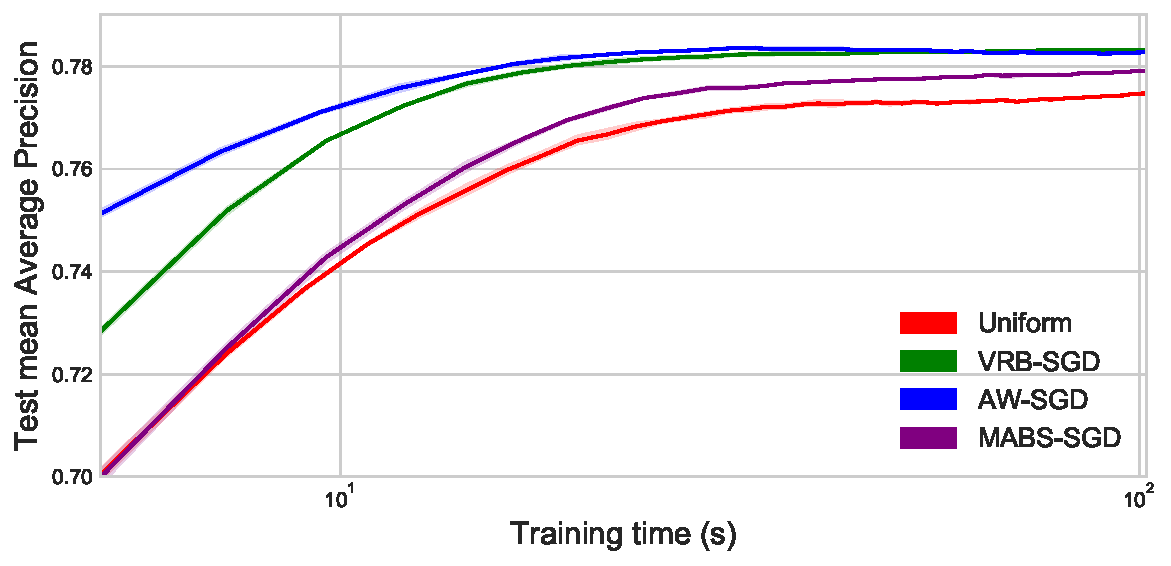
\includegraphics[width=\linewidth]{figures/voc-result.pdf}
      \caption{Mean Average Precision scores achieved on the test part of VOC 2007.}
      \label{fig:exp1}
\end{minipage}%
\quad
\begin{minipage}{.48\textwidth}
  \centering
  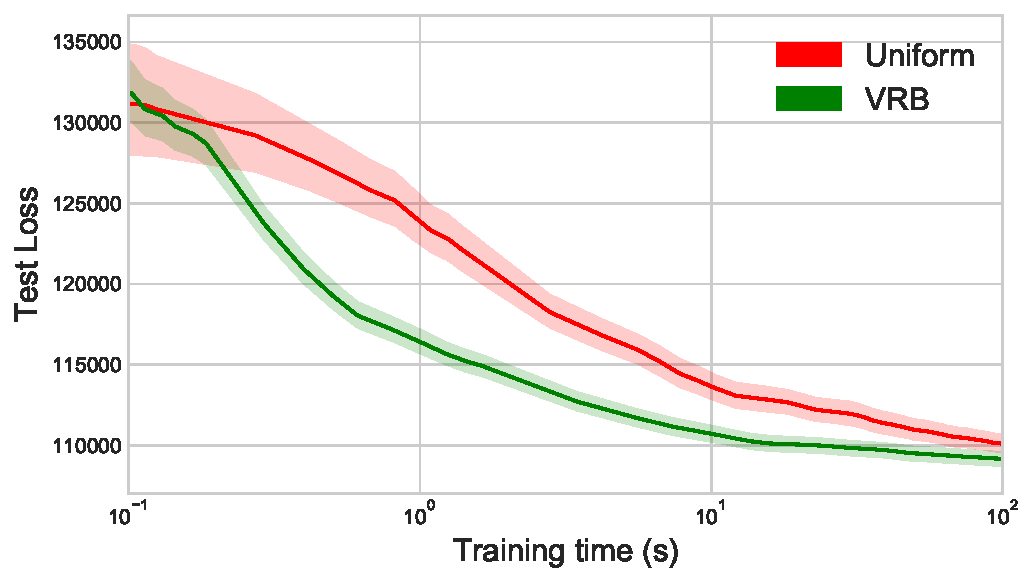
\includegraphics[width=.88\linewidth]{figures/kmeans-csn.pdf}
      \caption{$k$-Means test loss evolution on the CSN dataset.}
      \label{fig:exp2}
\label{fig:exp}
\end{minipage}%
\end{figure}

% % !TEX root = main.tex
\newpage
\section{Experiments} \label{sec:experiments}
\subsection{Image Classification}

Training a binary classifier with imbalanced data is a challenging task in machine learning. Practices for dealing with imbalance include optimizing class weight hyperparameters, hard negative mining \citep{shrivastava2016training} and synthetic minority oversampling \citep{chawla2002smote}. 
Without accounting for imbalance, the minority samples are often misclassified in early stages of the iterative training procedures, resulting in high loss and high gradient norms associated with these points. Importance sampling schemes for reducing the variance of the gradient norms will sample these instances more often at the early phases, offering a way of tackling imbalance.

For verifying this intuition, we perform the image classification experiment of \cite{bouchard2015online}. We train one-vs-all logistic regression Pascal VOC 2007 dataset \citep{everingham2010pascal} with image features extracted from the last layer of the VGG16 \citep{simonyan2014very} pretrained on Imagenet. We measure the average precision by reporting its mean over the 20 classes of the test data. The optimization is performed with AdaGrad \citep{duchi2011adaptive}, where learning rate is initialized to 0.1. The losses received by the bandit methods are the norms of the logistic loss gradient.
We compare our method, Variance Reducer Bandit (VRB), to:
\vspace{-1.5mm}
\begin{itemize}
\setlength\itemsep{0.05em}
\item uniform sampling for SGD,
\item Adaptive Weighted SGD (AW) \citep{bouchard2015online} ---  variance reduction by sampling from a chosen distribution whose parameters are optimized alternatingly with the model parameters,
\item MABS \citep{salehi2017} --- bandit algorithm for variance reduction that relies on EXP3 through employing modifies losses.  
\end{itemize}

\begin{figure}[h]
\centering
\begin{minipage}{.48\textwidth}
  \centering
  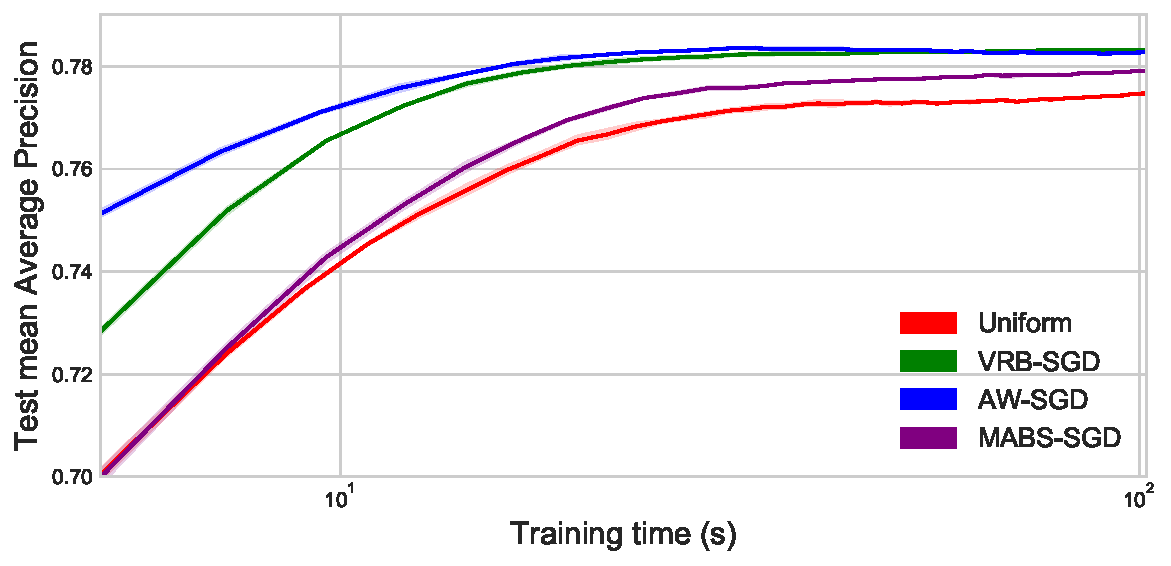
\includegraphics[width=\linewidth]{figures/voc-result.pdf}
      \caption{Mean Average Precisions on the test part of VOC 2007.}
      \label{fig:voc-results}
\end{minipage}%
\quad
\begin{minipage}{.48\textwidth}
  \centering
  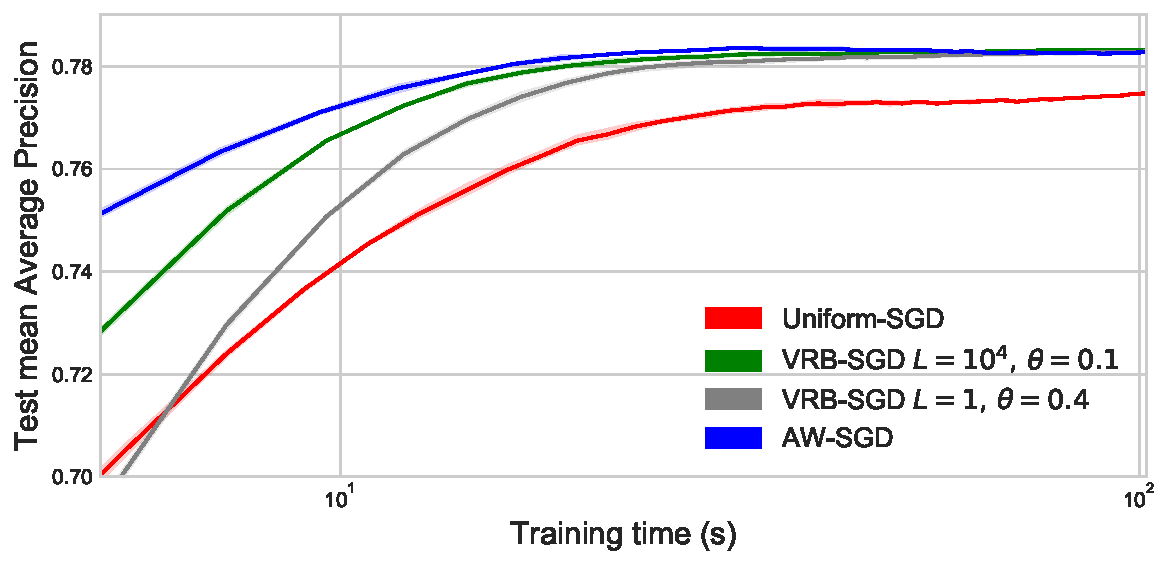
\includegraphics[width=\linewidth]{figures/voc-result-2.pdf}
      \caption{The effect of different hyperparameters on VRB. }
      \label{fig:voc-results-2}
\label{fig:test}
\end{minipage}%
\end{figure}

        
The hyperparameters of the methods are chosen based on cross-validation on the validation portion of the dataset. The results can be seen in Figure \ref{fig:voc-results}, where the shaded areas represent confidence $95\%$ intervals over 10 runs. The best performing method is AW, but its disadvantage compared to the bandit algorithms is that it requires choosing a family of sampling distributions, which usually incorporates prior knowledge, and calculating the derivative of the log-density. VRB and AW both outperform uniform subsampling with respect to the training time.  VRB performs similarly to AW at convergence, and speeds up training 10 times compared to uniform sampling, by attaining a certain score level 10 times faster. We have also experimented with the variance reduction method of \cite{pmlr-v70-namkoong17a}, but it did not outperform uniform sampling significantly. Since cross-validation is costly, in Figure \ref{fig:voc-results-2} we show the effect of the hyperparameters of our method. More specifically, we compare the performance of VRB with misspecified regularizer $L=1$ to the best $L=10^8$ chosen by cross-validation, and we compensate by using higher mixing coefficient $\theta=0.4$. The fact that only the early-stage performance is affected is a sign of method's robustness against regularizer misspecification.

We also measure the regret incurred both by the full information and VRB samplers, and show the results in Figure \ref{fig:regret}. For a fair comparison, we choose an \emph{oblivious} adversary that generates the loss sequences by performing the same optimization process as described above on a subset of 1000 data points from VOC 2007, with uniform sampling. For VRB, we report the average regret over 10 runs. 
\begin{figure}[h]

		\centering
		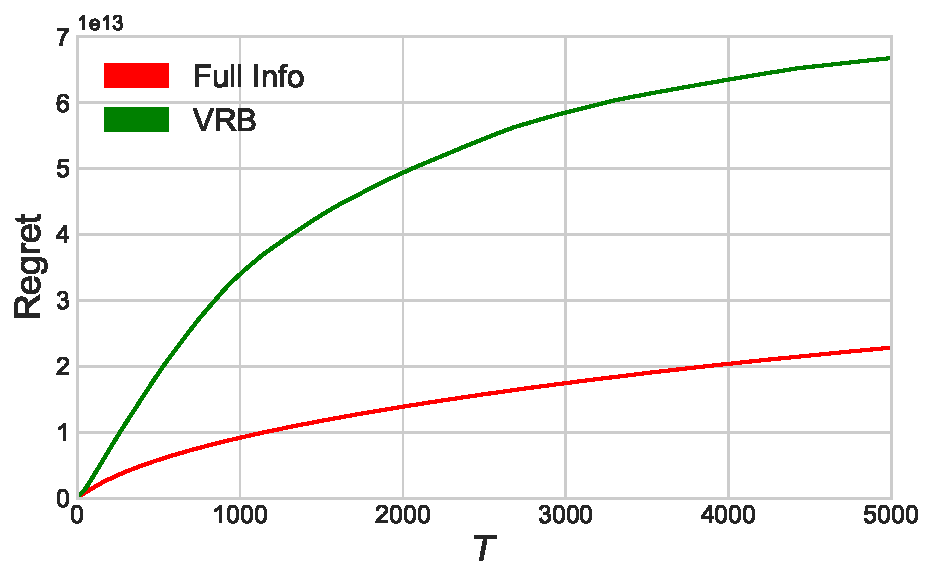
\includegraphics[width=0.5\linewidth]{figures/regret.pdf}
		\caption{Regret incurred by the full info and VRB.}
		\label{fig:regret}
\end{figure}


\subsection{$k$-Means}

In this experiment, we show that in some applications it is beneficial to work with per-sample upper bound estimates $L_i$ instead of a single global bound. As an illustrative example, we choose mini-batch $k$-Means clustering \citep{sculley2010web}. This is a slight deviation from the presented theory, since we sample multiple points for the batch and update the sampler only  once, upon observing the loss for the batch. 

In the case of $k$-Means, the parameters consist of the coordinates of the $k$ centers \linebreak $Q=\{q_1, q_2, \dots, q_k\}$. As the cost function for a point $x_i \in \{x_1, x_2, \dots, x_n \}$ is the  squared Euclidean distance to the closest center, the loss received by VRB  is the norm of the gradient  \linebreak $\min _{q \in Q } 2 \cdot || x_i - q||_2$. This lends itself to a natural estimation of $L_i$:
choose a point $u$ randomly from the dataset and define $L_i=4 \cdot || x_i - u||^2_2$. For this experiment, we set $\theta=0.5$.

We solve mini-batch $k$-Means  for $k=100$ and batch size $b=100$ with uniform sampling and VRB. The initial centers are chosen with $k$-Means++ \citep{arthur2007k} from a random subsample of 1000 points from the training data and they are shared between the methods. We generate 10 different sets of initial centers and run both algorithms 10 times on each set of centers, with different random seeds for the samplers.  We train the algorithm on $80 \%$ of the data, and measure the cost of the $20 \%$ test portion for the following datasets:
\vspace{-2mm}
\begin{itemize}
\setlength\itemsep{0.2em}
  \item \texttt{CSN} \citep{faulkner2011next} --- cellphone accelerometer with 80,000 observations and 17 features,
 \item \texttt{KDD} \citep{kddcup2004} --- data set used for Protein Homology Prediction KDD
    competition  containing 145,751 observations with 74 features,
    \item \texttt{MNIST} \citep{lecun1998gradient} --- 70,000 low resolution images of handwritten
    characters transformed using PCA with whitening and retaining 10 dimensions.  
\end{itemize}

\begin{figure}[h]
      \centering
      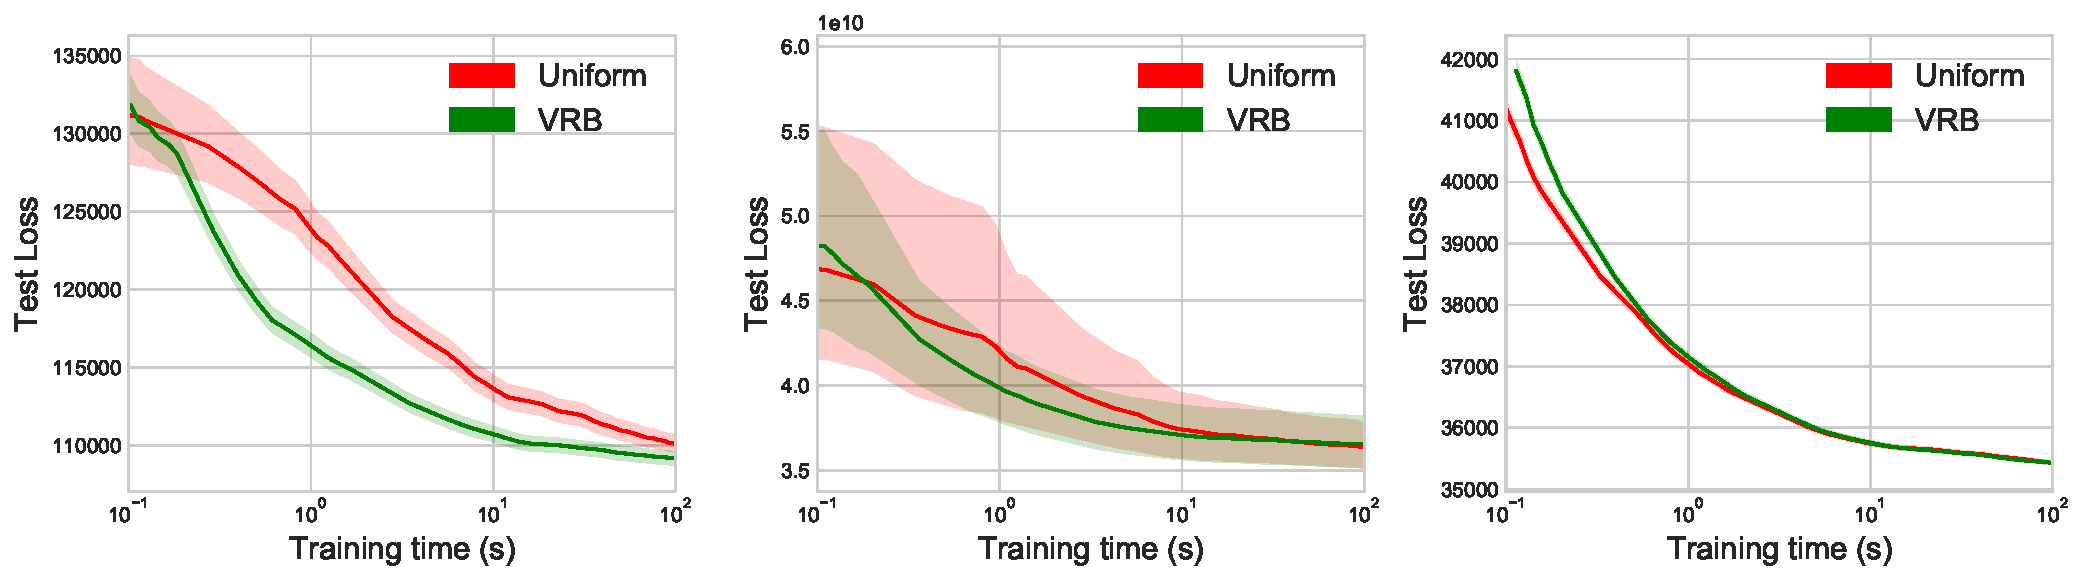
\includegraphics[width=\linewidth]{figures/kmeans.pdf}
      \caption{The evolution of the loss of $k$-Means on the test set. The shaded areas represent $95\%$ confidence intervals over 100 runs.}
      \label{fig:kmeans-results}
        \end{figure}
        
The evolution of the cost function on the test set with respect to the elapsed training time is shown in Figure \ref{fig:kmeans-results}. The chosen datasets illustrate three observed behaviors of our algorithm. In the case of \texttt{CSN}, our method significantly outperforms uniform subsampling. In the case of \texttt{KDD}, the advantage of our method can be seen in the reduced variance of the cost over multiple runs, whereas on \texttt{MNIST} we observe no advantage.
This behavior is highly dependent on intrinsic dataset characteristics: for \texttt{MNIST}, we note that the entropy of the best-in-hindsight sampling distribution is close the entropy of the uniform distribution. We have also compared VRB with the bandit algorithms mentioned in the previous section. Since mini-batch $k$-Means converges in 1-2 epochs, these methods with  uniform initialization do not outperform uniform subsampling significantly. Thus, for this setting, careful initialization is necessary, which is naturally supported by our method.

% !TEX root = main.tex

\section{Conclusions}

In this paper, we showed that even though non-convex approaches for matrix completion are not robust in the semi-random model, but it is possible to fix them using a pre-processing step.
The pre-processing step solves a few convex programs (packing SDPs) to ameliorate the influence of the semi-random adversary. %, and produces a weighted instance with spectral properties similar to a random graph.
Unlike the full convex relaxation for matrix completion, our pre-processing step runs in nearly-linear time. Combining our pre-processing step with non-convex optimization gives an algorithm that is robust in the semi-random model, and at the same time enjoys the efficiency of the non-convex approaches.

%Our pre-processing step solves a variant of the graph sparsification problem.
%Given a graph $G$ formed by adding extra edges to $H$ (or a graph similar to $H$), we can produce a weighted version of $G$ that is spectrally similar to $H$.
%We believe this subroutine can be useful in other problems.

An immediate open problem is whether we can prove the output of the pre-processing step allows non-convex optimization to recover the ground truth {\em exactly}.
%This would require proving stronger concentration inequalities like Lemma~\ref{lem:tangent} using deterministic conditions.
More broadly, we hope this work will inspire new ideas that make non-convex optimization more robust.

% Acknowledgments---Will not appear in anonymized version
\acks{The authors would like  to thank  
Hasheminezhad Seyedrouzbeh  for useful discussions during the course of this work. This research was supported by SNSF grant $407540\_167212$ through the NRP 75 Big Data program.
K.Y.L. is supported by the ETH Z\"urich Postdoctoral Fellowship and Marie Curie Actions for People COFUND program.}

\newpage
\bibliography{bib}
\appendix

\section{Proof of Lemma \ref{thm:general_instantaneous}}
\begin{proof}{\textbf{of Lemma \ref{thm:general_instantaneous}}.}
We first state a useful property used in typical OMD analysis. Let $\Omega$ be a convex compact set in $\mathbb{R}^K$, $\psi$ be a convex function on $\Omega$, 
$w'$ be an arbitrary point in $\Omega$, and $x \in \mathbb{R}^K$.
If $w^*=\argmin_{w\in \Omega}\{\inn{w,x}+D_{\psi}(w,w')\}$, then for any $u \in \Omega$,
\begin{align*}
\inn{w^*-u, x}\leq D_{\psi}(u,w')-D_\psi(u,w^*)-D_{\psi}(w^*,w'). 
\end{align*}
This is by the first-order optimality condition of $w^*$ and direct calculations. Applying this to update rule~\eqref{eqn:update_rule_2} we have
\begin{align}
\inn{w_{t+1}^\p-u, \hat{\ell}_t+ a_t} \leq D_{\psi_t}(u,w_{t}^\p)-D_{\psi_t}(u,w_{t+1}^\p)-D_{\psi_t}(w_{t+1}^\p, w_{t}^\p); \label{eqn:apply1}
\end{align}
while applying it to update rule~\eqref{eqn:update_rule_1} and picking $u=w_{t+1}^\p$ we have
\begin{align}
\inn{w_t-w_{t+1}^\p, m_t} \leq D_{\psi_t}(w_{t+1}^\p, w_t^\p)-D_{\psi_t}(w_{t+1}^\p, w_t)-D_{\psi_t}(w_t, w_t^\p).\label{eqn:apply2} 
\end{align}
Now we bound the instantaneous regret as follows:
\begin{align}
&\inn{w_t-u, \hat{\ell}_t}\nonumber \\
&=\inn{w_t-u, \hat{\ell}_t+ a_t}-\inn{w_t, a_t}+\inn{u,  a_t}\nonumber \\
&=\inn{w_t-w_{t+1}^\p, \hat{\ell}_t+a_t}-\inn{w_t, a_t}+\inn{w_{t+1}^\p-u, \hat{\ell}_t+a_t}+\inn{u,   a_t}\nonumber \\
&=\inn{w_t-w_{t+1}^\p, \hat{\ell}_t+a_t-m_t}-\inn{w_t,a_t}+\inn{w_{t+1}^\p-u, \hat{\ell}_t+ a_t}+\inn{w_t-w_{t+1}^\p, m_t}+\inn{u,   a_t} \nonumber \\
&\leq D_{\psi_t}(u,w_{t}^\p)-D_{\psi_t}(u,w_{t+1}^\p)-D_{\psi_t}(w_{t+1}^\p, w_t)-D_{\psi_t}(w_t, w_t^\p)+\inn{u, a_t}, \label{eqn:regret_decomposition}
\end{align}
where last inequality is by the condition $\inn{w_t-w_{t+1}^\p, \hat{\ell}_t+a_t-m_t}-\inn{w_t,a_t}\leq 0$, Eq.~\eqref{eqn:apply1}, and Eq.~\eqref{eqn:apply2}.
\end{proof}

\section{Lemmas for Log-barrier OMD}
\label{section:all_kinds_of_lemmas}

In this section we establish some useful lemmas for update rules~\eqref{eqn:update_rule_1} and~\eqref{eqn:update_rule_2} with log-barrier regularizer,
which are used in the proofs of other theorems.
We start with some definitions.

\begin{definition}
\label{definition:norm}
For any $h \in \mathbb{R}^K$, define norm $\norm{h}_{t,w}=\sqrt{h^\top \nabla^2 \psi_t(w) h}=\sqrt{\sum_{i=1}^K \frac{1}{\eta_{t,i}}\frac{h_i^2}{w_i^2}}$ and its dual norm $\norm{h}_{t,w}^*=\sqrt{h^\top \nabla^{-2} \psi_t(w) h}=\sqrt{\sum_{i=1}^K \eta_{t,i}w_i^2 h_i^2}$.
For some radius $r > 0$, define ellipsoid $\mathcal{E}_{t,w}(r)=\left\{u \in \mathbb{R}^K : \norm{u-w}_{t,w}\leq r \right\}$ . 
\end{definition}

\begin{lemma}
\label{lemma:norm_close}
If $w^\p \in \mathcal{E}_{t,w}(1)$ and $\eta_{t,i}\leq \frac{1}{81}$ for all $i$, then $w_i^\p\in \left[ \frac{1}{2}w_i, \frac{3}{2}w_i \right]$ for all $i$, and also $ 0.9\norm{h}_{t,w} \leq \norm{h}_{t,w^\p} \leq 1.2\norm{h}_{t,w}$ for any $h\in \mathbb{R}^K$. 
\end{lemma}
\begin{proof}
$w^\p\in \mathcal{E}_{t,w}(1)$ implies $\sum_{i=1}^K \frac{1}{\eta_{t,i}}\frac{(w^\p_i-w_i)^2}{w_i^2}\leq 1$. Thus for every $i$, we have $\frac{\abs{w_i^\p-w_i}}{w_i}\leq \sqrt{\eta_{t,i}}\leq \frac{1}{9}$, implying $w_i^\p\in \left[ \frac{8}{9}w_i, \frac{10}{9}w_i \right]\subset\left[ \frac{1}{2}w_i, \frac{3}{2}w_i \right]$. 
Therefore, $\norm{h}_{t,w^\p}
=\sqrt{\sum_{i=1}^K \frac{1}{\eta_{t,i}} \frac{h_i^2}{w^{\p 2}_i}}
\geq \sqrt{\sum_{i=1}^K \frac{1}{\eta_{t,i}}\frac{h_i^2}{\left(\frac{10}{9}w_i\right)^2}}
=0.9\norm{h}_{t,w}$. 
Similarly, we have $\norm{h}_{t,w^\p}\leq 1.2\norm{h}_{t,w}$. 
\end{proof}

\begin{lemma}
\label{lemma:stability}
Let $w_t, w_{t+1}^\p$ follow \eqref{eqn:update_rule_1} and \eqref{eqn:update_rule_2} where $\psi_t$ is the log-barrier with $\eta_{t,i}\leq \frac{1}{81}$ for all $i$. If $\norm{\hat{\ell}_t-m_t+a_t}^*_{t,w_t}\leq \frac{1}{3}$, then $w_{t+1}^\p \in \mathcal{E}_{t,w_t}(1)$. 
\end{lemma}

\begin{proof}
Define $F_{t}(w)=\inn{w, m_t}+D_{\psi_t}(w, w_t^\p)$ and $F_{t+1}^\p(w)=\inn{w, \hat{\ell}_t+a_t}+D_{\psi_t}(w, w_t^\p)$. Then by definition we have $w_t=\argmin_{w\in\Omega}F_{t}(w)$ and $w_{t+1}^\p=\argmin_{w\in\Omega}F_{t+1}^\p(w)$. To show $w_{t+1}^\p\in \mathcal{E}_{t,w_t}(1)$, it suffices to show that for all $u$ on the boundary of $\mathcal{E}_{t,w_t}(1)$, $F^\p_{t+1}(u)\geq F^\p_{t+1}(w_t)$. 

Indeed, using Taylor's theorem, for any $u\in \partial \mathcal{E}_{t,w_t}(1)$, there is an $\xi$ on the line segment between $w_t$ and $u$ such that (let $h\triangleq u-w_t$)
\begin{align*}
F^\p_{t+1}(u)&=F^\p_{t+1}(w_t)+\nabla F^{\p}_{t+1} (w_t)^\top h+ \frac{1}{2}h^\top\nabla^2 F^\p_{t+1}(\xi)h \\
&=F^\p_{t+1}(w_t)+ (\hat{\ell}_t-m_t+a_t)^\top h +\nabla F_t (w_t)^\top h+ \frac{1}{2}h^\top\nabla^2 \psi_t(\xi)h \\
&\geq F^\p_{t+1}(w_t)+ (\hat{\ell}_t-m_t+a_t)^\top h + \frac{1}{2}\norm{h}_{t,\xi}^2 \tag{by the optimality of $w_t$}\\
&\geq F^\p_{t+1}(w_t)+ (\hat{\ell}_t-m_t+a_t)^\top h + \frac{1}{2}\times0.9^2\norm{h}_{t,w_t}^2 \tag{by Lemma \ref{lemma:norm_close}} \\
&\geq F^\p_{t+1}(w_t)- \norm{\hat{\ell}_t-m_t+a_t}^*_{t,w_t} \norm{h}_{t,w_t} + \frac{1}{3}\norm{h}_{t,w_t}^2 \\
&=F^\p_{t+1}(w_t)- \norm{\hat{\ell}_t-m_t+a_t}^*_{t,w_t} + \frac{1}{3} \tag{$\norm{h}_{t,w_t}=1$}\\
&\geq F^\p_{t+1}(w_t). \tag{by the assumption}
\end{align*}
\end{proof}

\begin{lemma}
\label{lemma:stability_under_condition}
Let $w_t, w_{t+1}^\p$ follow \eqref{eqn:update_rule_1} and \eqref{eqn:update_rule_2} where $\psi_t$ is the log-barrier with $\eta_{t,i}\leq \frac{1}{81}$ for all $i$. If $\norm{\hat{\ell}_t-m_t+a_t}^*_{t,w_t}\leq \frac{1}{3}$, then $\norm{w_{t+1}^\p-w_t}_{t,w_t}\leq 3\norm{\hat{\ell}_t-m_t+a_t}_{t,w_t}^*$. 
\end{lemma}
\begin{proof}
Define $F_t(w)$ and $F_{t+1}^\p(w)$ to be the same as in Lemma \ref{lemma:stability}. Then we have 
\begin{align}
F_{t+1}^\p(w_t)-F_{t+1}^\p(w_{t+1}^\p)&=(w_t-w_{t+1}^\p)^\top(\hat{\ell}_t-m_t+a_t) + F_t(w_t)-F_t(w_{t+1}^\p) \nonumber \\
&\leq (w_t-w_{t+1}^\p)^\top(\hat{\ell}_t-m_t+a_t) \nonumber \tag{optimality of $w_t$}\\
&\leq \norm{w_t-w_{t+1}^\p}_{t,w_t}\norm{\hat{\ell}_t-m_t+a_t}_{t,w_t}^*. \label{eqn:direction1}
\end{align}
On the other hand, for some $\xi$ on the line segment between $w_t$ and $w_{t+1}^\p$, we have by Taylor's theorem and the optimality of $w_{t+1}^\p$,
\begin{align}
F_{t+1}^\p(w_t)-F_{t+1}^\p(w_{t+1}^\p)&=\nabla F_{t+1}^\p(w_{t+1}^\p)^\top (w_t-w_{t+1}^\p) + \frac{1}{2}(w_t-w_{t+1}^\p)^\top \nabla^2 F_{t+1}^\p(\xi)(w_t-w_{t+1}^\p) \nonumber \\
&\geq \frac{1}{2}\norm{w_t-w_{t+1}^\p}_{t,\xi}^2 .
\label{eqn:direction2}
\end{align}
Since the condition in Lemma \ref{lemma:stability} holds, $w_{t+1}^\p\in \mathcal{E}_{t,w_t}(1)$, and thus $\xi\in \mathcal{E}_{t,w_t}(1)$. Using again Lemma \ref{lemma:norm_close}, we have 
\begin{align}
\frac{1}{2}\norm{w_t-w_{t+1}^\p}_{t,\xi}^2 \geq \frac{1}{3}\norm{w_t-w_{t+1}^\p}_{t,w_t}^2\label{eqn:direction3}.
\end{align}
Combining \eqref{eqn:direction1}, \eqref{eqn:direction2}, and \eqref{eqn:direction3}, we have $\norm{w_t-w_{t+1}^\p}_{t,w_t}\norm{\hat{\ell}_t-m_t+a_t}_{t,w_t}^* \geq \frac{1}{3}\norm{w_t-w_{t+1}^\p}_{t,w_t}^2$, which leads to the stated inequality. 
\end{proof}

\begin{lemma}
\label{lemma:condition_automatic_hold}
%Let $w_t, w_{t+1}^\p$ follow \eqref{eqn:update_rule_1} and \eqref{eqn:update_rule_2}. 
When the three conditions in Theorem \ref{lemma:MAB_condition} hold, we have $\norm{\hat{\ell}_t-m_t+a_t}^{*}_{t,w_t}\leq \frac{1}{3}$ for either $a_{t,i}=6\eta_{t,i}w_{t,i}(\hat{\ell}_{t,i}-m_{t,i})^2$ or $a_{t,i}=0$.  
\end{lemma}
\begin{proof}
For $a_{t,i}=6\eta_{t,i}w_{t,i}(\hat{\ell}_{t,i}-m_{t,i})^2$, we have
\begin{align*}
\norm{\hat{\ell}_t-m_t+a_t}^{*2}_{t,w_t}
&= \sum_{i=1}^K\eta_{t,i}w_{t,i}^2\big(\hat{\ell}_{t,i}-m_{t,i} + 6\eta_{t,i}w_{t,i}(\hat{\ell}_{t,i}-m_{t,i})^2\big)^2 \\
&=\sum_{i=1}^K\eta_{t,i}w_{t,i}^2(\hat{\ell}_{t,i}-m_{t,i})^2+12\eta_{t,i}^2w_{t,i}^3(\hat{\ell}_{t,i}-m_{t,i})^3 +36\eta_{t,i}^3w_{t,i}^4(\hat{\ell}_{t,i}-m_{t,i})^4\\
&\leq \sum_{i=1}^K \eta_{t,i}w_{t,i}^2(\hat{\ell}_{t,i}-m_{t,i})^2(1+36\eta_{t,i}+324\eta_{t,i}^2) \tag{condition (ii)}\\
&\leq 2\sum_{i=1}^K \eta_{t,i}w_{t,i}^2(\hat{\ell}_{t,i}-m_{t,i})^2 \tag{condition (i)}\\
&\leq 2\times \frac{1}{18}=\frac{1}{9}.\tag{condition (iii)}
\end{align*}
For $a_{t,i}=0$, we have
\begin{align*}
\norm{\hat{\ell}_t-m_t+a_t}^{*2}_{t,w_t}=\norm{\hat{\ell}_t-m_t}^{*2}_{t,w_t}=\sum_{i=1}^K \eta_{t,i}w_{t,i}^2(\hat{\ell}_{t,i}-m_{t,i})^2\leq \frac{1}{18} < \frac{1}{9}. \tag{condition (iii)}
\end{align*}
%When $a_{t,i}=0$,
%\begin{align*}
%\norm{\hat{\ell}_t-m_t+a_t}_{t,w_t}^{*2}= \sum_{i=1}^K \eta_{t,i}w_{t,i}^2(\hat{\ell}_{t,i}-m_{t,i})^2 \leq \frac{1}{18}<\frac{1}{9}. \text{\ \ \ \ \ \ \ \ \ \ \ \ \ \ \ \ \ \ \ \ \ \ \ (condition(iii))} 
%\end{align*}
\end{proof}

\begin{lemma}
\label{lemma:2times_bound}
If the three conditions in Theorem \ref{lemma:MAB_condition} hold, \textsc{Broad-OMD} (with either Option I or II)
satisfies $\frac{1}{2}w_{t,i}\leq w^\p_{t+1,i}\leq \frac{3}{2}w_{t,i}$.
%Let $w_t, w_{t+1}^\p$ follow \eqref{eqn:update_rule_1} and \eqref{eqn:update_rule_2}. If the three conditions in Theorem \ref{lemma:MAB_condition} hold, then $\frac{1}{2}w_{t,i}\leq w^\p_{t+1,i}\leq \frac{3}{2}w_{t,i}$, for either $a_{t,i}=6\eta_{t,i}w_{t,i}(\hat{\ell}_{t,i}-m_{t,i})^2$ or $a_{t,i}=0$.
\end{lemma}
\begin{proof}
This is a direct application of Lemmas \ref{lemma:condition_automatic_hold},  \ref{lemma:stability}, and \ref{lemma:norm_close}.
%It suffices to prove $w_{t+1}^\p \in \mathcal{E}_{t,w_t}(1)$, because if it is true, then
%\begin{align*}
%\norm{w_{t+1}^\p-w_t}_{t,w_t}=\sqrt{\sum_{i=1}^K\frac{1}{\eta_{t,i}}\frac{(w^\p_{t+1,i}-w_{t,i})^2}{w_{t,i}^2}}\leq 1, 
%\end{align*}
%which implies $\frac{\abs{w_{t+1,i}^\p-w_{t,i}}}{w_{t,i}}\leq \sqrt{\eta_{t,i}}\leq \frac{1}{2}$. Thus, $w_{t+1,i}^\p \in [\frac{1}{2}w_{t,i}, \frac{3}{2}w_{t,i}]$.

%Since we assume the three conditions in Theorem \ref{lemma:MAB_condition} hold, $w_{t+1}^\p \in \mathcal{E}_{t,w_t}(1)$ can be proved by applying Lemma \ref{lemma:condition_automatic_hold} and Lemma \ref{lemma:stability} back to back.

\end{proof}

\begin{lemma}
\label{lemma:2times_bound_another}
For the MAB problem, if the three conditions in Theorem \ref{lemma:MAB_condition} hold, \textsc{Broad-OMD} (with either Option I or II)
satisfies $\frac{1}{2}w_{t,i}\leq w^\p_{t,i}\leq \frac{3}{2}w_{t,i}$.
\end{lemma}
\begin{proof}
It suffices to prove $w_{t}^\p \in \mathcal{E}_{t,w_t}(1)$ by Lemma~\ref{lemma:norm_close}.
Since we assume that the three conditions in Theorem \ref{lemma:MAB_condition} hold and $w_t\in \Delta_K$, we have $\norm{m_t}_{t,w_t}^*=\sqrt{\sum_{i=1}^K \eta_{t,i}w_{t,i}^2m_{t,i}^2}\leq \sqrt{\frac{1}{162}\sum_{i=1}^K w_{t,i}^2}\leq \sqrt{\frac{1}{162}}< \frac{1}{3}$. This implies $w_{t}^\p \in \mathcal{E}_{t,w_t}(1)$ by a similar arguments as in the proof of Lemma~\ref{lemma:stability} (one only needs to replace $F_{t+1}^\p(w)$ there by $G(w)\triangleq D_{\psi_t}(w,w_t^\p)$ and note that $w_t^\p=\argmin_{w\in \Delta_K}G(w)$).
\end{proof}


%\begin{lemma}
%\label{lemma:stability_game}
%For MAB problems, if the three conditions in Theorem \ref{lemma:MAB_condition} hold, then \textsc{Broad-OMD} with $a_{t,i}=\mathbf{0}$ and fixed learning rate $\eta$ guarantees $\norm{w_{t+1}-w_t}_1 = \mathcal{O}(\eta)$ for all $t$.  
%\end{lemma}
%\begin{proof}
%By Lemma \ref{lemma:condition_automatic_hold} and \ref{lemma:stability_under_condition}, we have $\norm{w_t-w_{t+1}^\p}_{t,w_t}\leq 3\norm{\hat{\ell}_t-m_t}_{t,w_t}^*$, which implies
%\begin{align*}
%\frac{1}{\eta}\frac{(w_{t,j}-w_{t+1,j}^\p)^2}{w_{t,j}^2}\leq \sum_{i=1}^K\frac{1}{\eta}\frac{(w_{t,i}-w_{t+1,i}^\p)^2}{w_{t,i}^2}\leq 3\eta\sum_{i=1}^K  w_{t,i}^2(\hat{\ell}_{t,i}-m_{t,i})^2\leq 3\eta\times 9. 
%\end{align*}
%Therefore, $\abs{w_{t,j}-w_{t+1,j}^\p} = \mathcal{O}(\eta w_{t,j})$. We can use similar techniques in Lemma \ref{lemma:condition_automatic_hold} and \ref{lemma:stability_under_condition} to prove $\norm{w_{t+1}-w_{t+1}^\p}_{t,w_{t+1}^\p}\leq 3\norm{m_{t+1}}_{t,w_{t+1}^\p}^*$, and thus  $\abs{w_{t+1,j}^\p-w_{t+1,j}}=\mathcal{O}(\eta w_{t+1,j}^\p)=\mathcal{O}(\eta w_{t,j})$. Thus, $\abs{w_{t,j}-w_{t+1,j}}=\mathcal{O}(\eta w_{t,j})$, which implies $\norm{w_t-w_{t+1}}_1=\mathcal{O}(\eta)$. 
%\end{proof}

\section{Proof of Theorem \ref{lemma:MAB_condition} and Corollary~\ref{cor:clear_corollary}}
%To prove Theorem \ref{lemma:MAB_condition}, we need some definitions and lemmas established in Section~\ref{section:all_kinds_of_lemmas}. 

\begin{proof}{\textbf{of Theorem \ref{lemma:MAB_condition}}.}
We first prove Eq.~\eqref{eqn:condition1} holds: by Lemmas \ref{lemma:condition_automatic_hold} %, we have $\norm{\hat{\ell}_t-m_t+a_t}^{*}_{t,w_t}\leq \frac{1}{3}$. Then by
and \ref{lemma:stability_under_condition}, we have
\begin{align*}
\inn{w_t-w_{t+1}^\p, \hat{\ell}_t-m_t+ a_t}
&\leq \norm{w_t-w_{t+1}^\p}_{t,w_t}\norm{\hat{\ell}_t-m_t+a_t}_{t,w_t}^*\\
&\leq 3\norm{\hat{\ell}_t-m_t+a_t}_{t,w_t}^{*2}\\
&\leq 3\sum_{i=1}^K \eta_{t,i}w_{t,i}^2(\hat{\ell}_{t,i}-m_{t,i})^2(1+36\eta_{t,i}+324\eta_{t,i}^2) \\
&\leq 6\sum_{i=1}^K \eta_{t,i}w_{t,i}^2(\hat{\ell}_{t,i}-m_{t,i})^2 = \inn{w_t, a_t},
\end{align*}
where the last two inequalities are by the same calculations done in the proof of Lemma~\ref{lemma:condition_automatic_hold}.
%where $C=6$. With our choice of $C$ and $\eta_{t,i}$, we have $3(1+6\eta_{t,i}C+9\eta_{t,i}^2C^2)\leq 3\left(1+6\times\frac{6}{162}+9\times \left(\frac{6}{162}\right)^2\right)\leq C$. Therefore, the last expression is further bounded by $\sum_{i=1}^K C\eta_{t,i}w_{t,i}^2(\hat{\ell}_{t,i}-m_{t,i})^2$, which is equal to $\inn{w_t, a_t}$. 

Since Eq.~\eqref{eqn:condition1} holds, using Lemma~\ref{thm:general_instantaneous} we have (ignoring non-positive terms $-A_t$'s),
\begin{align}
\sum_{t=1}^T\inn{w_t-u, \hat{\ell}_t}&\leq \sum_{t=1}^T\left(D_{\psi_t}(u,w_t^\p)-D_{\psi_t}(u,w^\p_{t+1})\right)+\sum_{t=1}^T\inn{u,a_t}\nonumber \\
&\leq D_{\psi_1}(u, w_1^\p) + \sum_{t=1}^{T}\left( D_{\psi_{t+1}}(u, w^\p_{t+1})-D_{\psi_{t}}(u, w^\p_{t+1}) \right)+\sum_{t=1}^T\inn{u,a_t}.\label{eqn:some_intermediate}
\end{align}
In the last inequality, we add a term $D_{\psi_{T+1}}(u, w_{T+1}^\p) \geq 0$ artificially. As mentioned, $\psi_{T+1}$, defined in terms of $\eta_{T+1,i}$, never appears in the \textsc{Broad-OMD} algorithm. We can simply pick any $\eta_{T+1,i} > 0$ for all $i$ here. This is just to simplify some analysis later. 

The first term in \eqref{eqn:some_intermediate} can be bounded by the optimality of $w_1^\p$:
\begin{align*}
D_{\psi_1}(u, w_1^\p)&=\psi_1(u)-\psi_1(w_1^\p)-\inn{\nabla\psi_1(w_1^\p), u-w_1^\p}\\
&\leq \psi_1(u)-\psi_1(w_1^\p)=\sum_{i=1}^K \frac{1}{\eta_{1,i}}\ln\frac{w_{1,i}^\p}{u_i}.
\end{align*}
%where the inequality is because $w_1^\p$ is the minimizer of $\psi_1$. 
The second term, by definition, is
\begin{align*}
\sum_{t=1}^{T}\sum_{i=1}^K \left(\frac{1}{\eta_{t+1,i}}-\frac{1}{\eta_{t,i}}\right) h\left(\frac{u_i}{w_{t+1,i}^\p}\right). 
\end{align*}
Plugging the above two terms into \eqref{eqn:some_intermediate} finishes the proof.
\end{proof}

\begin{proof}{\textbf{of Corollary~\ref{cor:clear_corollary}}.}
We first check the three conditions in Theorem~\ref{lemma:MAB_condition} under our choice of $\eta_{t,i}$ and $\hat{\ell}_{t,i}$: $\eta_{t,i}=\eta=\frac{1}{162K_0}\leq \frac{1}{162}$; $w_{t,i}\abs{\hat{\ell}_{t,i}-m_{t,i}}=\abs{\ell_{t,i}-m_{t,i}}\mathbbm{1}\{i\in b_t\} \leq 2<3$; 
$\sum_{i=1}^K \eta_{t,i}w_{t,i}^2(\hat{\ell}_{t,i}-m_{t,i})^2=\frac{1}{162K_0}\sum_{i=1}^K (\ell_{t,i}-m_{t,i})^2\mathbbm{1}\{i\in b_t\} \leq \frac{4}{162} < \frac{1}{18}$. 
%(in the MAB case, $\sum_{i=1}^K \eta_{t,i}w_{t,i}^2(\hat{\ell}_{t,i}-m_{t,i})^2=\eta_{t,i_t}(\ell_{t,i_t}-m_{t,i_t})^2\leq \frac{1}{162}\times 3^2=\frac{1}{18}$). 
Applying Theorem~\ref{lemma:MAB_condition} we then have 
\begin{align*}
\sum_{t=1}^T \inn{w_t-u, \hat{\ell}_t}\leq \sum_{i=1}^K  \frac{\ln\frac{w^\p_{1,i}}{u_i}}{\eta}  +\sum_{t=1}^T \inn{u,a_t}.
\end{align*}
As mentioned, if we let $u=b^*$, then $\ln \frac{w_{1,i}^\p}{u_i}$
becomes infinity for those $i\notin b^*$. Instead, we let $u=\left(1-\frac{1}{T}\right)b^* + \frac{1}{T}w_1^\p$. With this choice of $u$, we have $\frac{w_{1,i}^\p}{u_i}\leq \frac{w_{1,i}^\p}{\frac{1}{T}w_{1,i}^\p}=T$. Plugging $u$ into the above inequality and rearranging, we get 
\begin{align}
\sum_{t=1}^T \inn{w_t-b^*, \hat{\ell}_t}\leq \frac{K\ln T}{\eta}+\sum_{t=1}^T \inn{b^*,a_t}+B,  \label{eqn:sb_corollary}
\end{align}
where $B\triangleq \frac{1}{T}\sum_{t=1}^T \inn{-b^*+w_1^\p, \hat{\ell}_t+a_t}$. 

Now note that $\mathbb{E}_{b_t}[a_{t,i}]=6\eta (\ell_{t,i}-m_{t,i})^2=\mathcal{O}(\eta)$ and $\mathbb{E}_{b_t}[\hat{\ell}_{t,i}]=\ell_{t,i}=\mathcal{O}(1)$ for all $i$. Thus, $\mathbb{E}[B]=\mathbb{E}\left[\frac{1}{T}\sum_{t=1}^T \inn{-b^*+w_1^\p, \mathbb{E}_{b_t}[\hat{\ell}_t+a_t]}\right] \leq \mathbb{E}\left[\frac{1}{T}\sum_{t=1}^T \norm{-b^*+w_1^\p}_1 \norm{\mathbb{E}_{b_t}[\hat{\ell}_t+a_t]}_\infty\right] = \mathcal{O}(K_0)$. Taking expectation on both sides of \eqref{eqn:sb_corollary}, we have 
\begin{align*}
\mathbb{E}\left[\sum_{t=1}^T b_t^\top \ell_t  - \sum_{t=1}^T b^{*\top} \ell_t \right] \leq \frac{K\ln T}{\eta} + 6\eta\mathbb{E}\left[\sum_{t=1}^T \sum_{i\in b^*}^K (\ell_{t,i}-m_{t,i})^2\right] + \mathcal{O}(K_0). 
\end{align*}
%One can verify that in the MAB case, the last term can be $\mathcal{O}(1)$ because now $b^*, w_1^\p \in \Delta_K$.  
\end{proof}

\section{Proof of Theorem \ref{cor:variance_bound}}
\begin{proof}{\textbf{of Theorem \ref{cor:variance_bound}}.}
As in \cite{hazan2011better}, 
for the rounds we perform uniform sampling we do not update $w_t^\p$. 
Let $\mathcal{S}$ be the set of rounds of uniform sampling. %Then in all other rounds the learner is essentially running an untouched \textsc{Broad-OMD}. Therefore, we can use Corollary \ref{cor:clear_corollary} to bound the regret. By Corollary \ref{cor:clear_corollary}, 
Then for the other rounds we can apply Corollary \ref{cor:clear_corollary} to arrive at
\begin{align}
\mathbb{E}\left[\sum_{t\in [T]\backslash \mathcal{S}} \ell_{t,i_t}-\ell_{t,i^*} \right]\leq \frac{K\ln T}{\eta} + 6\eta \mathbb{E}\left[\sum_{t\in [T]\backslash \mathcal{S}}(\ell_{t,i^*}-\tilde{\mu}_{t-1,i^*})^2\right] + \mathcal{O}(1). \label{eqn:regret_bound:a_t_neq_0_another} 
\end{align}
The second term can be bounded as follows: 
\begin{align}
&\mathbb{E}\left[\sum_{t\in [T]\backslash \mathcal{S}} (\ell_{t,i^*}-\tilde{\mu}_{t-1,i^*})^2\right]\leq \mathbb{E}\left[\sum_{t=2}^T (\ell_{t,i^*}-\tilde{\mu}_{t-1,i^*})^2\right] \nonumber \\
&\leq 3\sum_{t=2}^T(\ell_{t,i^*}-\mu_{t,i^*})^2+3\sum_{t=2}^T(\mu_{t,i^*}-\mu_{t-1,i^*})^2 + 3\mathbb{E}\left[\sum_{t=2}^T(\mu_{t-1,i^*}-\tilde{\mu}_{t-1,i^*})^2\right].\label{eqn:decompose_three}
\end{align}
The first and the third terms in \eqref{eqn:decompose_three} can be bounded using Lemma 10 and 11 of \citep{hazan2011better} respectively, and they are both of order $\mathcal{O}(Q_{T,i^*}+1)$ if we pick $M=\Theta(\ln T)$. The second term in \eqref{eqn:decompose_three} can be bounded by a constant by Lemma \ref{lemma:second_Q_term}. Thus second term in \eqref{eqn:regret_bound:a_t_neq_0_another}  can be bounded by $\mathcal{O}\left(\eta (Q_{T,i^*}+1)\right)$. Finally, note that $\mathbb{E}\left[\sum_{t=1}^T \ell_{t,i_t}-\ell_{t,i^*} \right]\leq\mathbb{E}\left[\sum_{t\in [T]\backslash \mathcal{S}} \ell_{t,i_t}-\ell_{t,i^*} \right]+2\mathbb{E}[\abs{\mathcal{S}}]$ and that $\mathbb{E}[\abs{\mathcal{S}}]=\mathcal{O}\left(\sum_{t=1}^T \frac{MK}{t}\right)=\mathcal{O}\left(MK\ln T\right)=\mathcal{O}\left(K(\ln T)^2\right)$. Combining everything, we get 
\begin{align*}
\mathbb{E}\left[\sum_{t=1}^T \ell_{t,i_t}-\ell_{t,i^*} \right]=\mathcal{O}\left( \frac{K\ln T}{\eta} + \eta Q_{T,i^*} + K(\ln T)^2\right).
\end{align*}
\end{proof}

\begin{lemma}
\label{lemma:second_Q_term}
For any $i$, $\sum_{t=2}^T (\mu_{t,i}-\mu_{t-1,i})^2=\mathcal{O}(1)$. 
\end{lemma}
\begin{proof}
By definition, \sloppy$\absolute{\mu_{t,i}-\mu_{t-1,i}}=\absolute{\frac{1}{t}\sum_{s=1}^t \ell_{s,i}-\frac{1}{t-1}\sum_{s=1}^{t-1} \ell_{s,i}}=\absolute{\frac{1}{t}\ell_{t,i}-\frac{1}{t(t-1)}\sum_{s=1}^{t-1}\ell_{s,i}}\leq \absolute{\frac{1}{t}\ell_{t,i}}+\absolute{\frac{1}{t(t-1)}\sum_{s=1}^{t-1}\ell_{s,i}}\leq \frac{2}{t}$. Therefore, $\sum_{t=2}^T (\mu_{t,i}-\mu_{t-1,i})^2\leq \sum_{t=2}^T \frac{4}{t^2}=\mathcal{O}(1)$. 
\end{proof}

\section{Proof of Theorem \ref{thm:path_length}}
We first state a useful lemma.
\begin{lemma}
\label{lemma:bound_ni}
Let $n_i$ be such that $\eta_{T+1,i}=\kappa^{n_i}\eta_{1,i}$, i.e., the number of times the learning rate of arm $i$ changes in \textsc{Broad-OMD+}. Then $n_i\leq \log_2 T$, and $\eta_{t,i}\leq 5\eta_{1,i}$ for all $t,i$.  
\end{lemma}
\begin{proof}
Let $t_1, t_2, \ldots, t_{n_i}\in [T]$ be the rounds the learning rate for arm $i$ changes (i.e., $\eta_{t+1,i}=\kappa \eta_{t,i}$ for $t=t_1, \ldots, t_{n_i}$). 
By the algorithm, we have 
\begin{align*}
KT\geq \frac{1}{\bar{w}_{t_{n_i},i}}>\rho_{t_{n_i},i}>2\rho_{t_{n_i-1},i}>\cdots>2^{n_i-1}\rho_{t_1,i}=2^{n_i}K. 
\end{align*}
Therefore, $n_i\leq \log_2 T$. And we have $\eta_{t,i}\leq \kappa^{\log_2 T}\eta_{1,i}=e^{\frac{\log_2 T}{\ln T}}\eta_{1,i}\leq 5\eta_{1,i}$.
\end{proof}




\begin{proof}{\textbf{of Theorem \ref{thm:path_length}}.}
Again, we verify the three conditions stated in Theorem \ref{lemma:MAB_condition}. By Lemma \ref{lemma:bound_ni}, $\eta_{t,i}\leq 5\eta\leq 5\times\frac{1}{810}=\frac{1}{162}$; also, $w_{t,j}\absolute{\hat{\ell}_{t,j}-m_{t,j}}=w_{t,j}\absolute{\frac{(\ell_{t,j}-m_{t,j})\mathbbm{1}\{i_t=j\}}{\bar{w}_{t,j}}}\leq w_{t,j}\absolute{\frac{2}{w_{t,j}\left(1-\frac{1}{T}\right)}}\leq 3$ because we assume $T\geq 3$; finally, $
\sum_{j=1}^K \eta_{t,j}w_{t,j}^2(\hat{\ell}_{t,j}-m_{t,j})^2=\eta_{t,i_t}w_{t,i_t}^2(\hat{\ell}_{t,i_t}-m_{t,i_t})^2\leq \frac{1}{162}\times 3^2=\frac{1}{18}$.

Let $\tau_j$ denote the last round the learning rate for arm $j$ is updated, that is, $\tau_j\triangleq \max\{t\in [T]: \eta_{t+1,j}=\kappa\eta_{t,j} \}$. 
We assume that the learning rate is updated at least once so that $\tau_j$ is well defined, otherwise one can verify that the bound is trivial.
For any arm $i$ to compete with, let 
$u=\left(1-\frac{1}{T}\right)\mathbf{e}_{i}+\frac{1}{T}w_1^\p
=\left(1-\frac{1}{T}\right)\mathbf{e}_{i}+\frac{1}{KT}\mathbf{1}$, which guarantees $\frac{w_{1,i}^\p}{u_i}\leq T$. Applying Theorem \ref{lemma:MAB_condition}, with $B\triangleq \frac{1}{T}\sum_{t=1}^T \inn{-\mathbf{e}_{i}+w^\p_{1}, \hat{\ell}_t+a_t}$ we have
\begin{align}
\sum_{t=1}^T\inn{w_t, \hat{\ell}_t}-\hat{\ell}_{t,i}&\leq \frac{K\ln T}{\eta} + \sum_{t=1}^{T}\sum_{j=1}^K\left(\frac{1}{\eta_{t+1,j}}-\frac{1}{\eta_{t,j}}\right)h\left(\frac{u_{j}}{w_{t+1,j}^\p}\right)+\sum_{t=1}^T a_{t,i}+B\nonumber \\
&\leq \frac{K\ln T}{\eta} + \left(\frac{1}{\eta_{\tau_i+1,i}}-\frac{1}{\eta_{\tau_i,i}}\right)h\left(\frac{u_{i}}{w_{\tau_i+1,i}^\p}\right)+\sum_{t=1}^T a_{t,i}+B\nonumber \\
&\leq \frac{K\ln T}{\eta} + \frac{1-\kappa}{\eta_{\tau_i+1,i}}h\left(\frac{u_{i}}{w_{\tau_i+1,i}^\p}\right)+\sum_{t=1}^T a_{t,i}+B\nonumber \\
&\leq \frac{K\ln T}{\eta} - \frac{1}{5\eta \ln T}h\left(\frac{u_{i}}{w_{\tau_i+1,i}^\p}\right)+\sum_{t=1}^T a_{t,i}+B,  \label{eqn:quasi_regret_bound1}
\end{align}
where the last inequality is by Lemma~\ref{lemma:bound_ni} and the fact $\kappa-1 \geq \frac{1}{\ln T}$. Now we bound the second and the third term in \eqref{eqn:quasi_regret_bound1} separately. 
\begin{enumerate}
\item For the second term,  by Lemma \ref{lemma:2times_bound} and $T \geq 3$ we have
\begin{align*}
\frac{u_{i}}{w^\p_{\tau_i+1,i}} \geq \frac{1-\frac{1}{T}}{ \frac{3}{2}w_{\tau_i, i} }\geq \frac{\left(1-\frac{1}{T}\right)^2}{\frac{3}{2}\bar{w}_{\tau_i,i}} =\frac{\left(1-\frac{1}{T}\right)^2}{\frac{3}{2}}\times \frac{\rho_{T+1,i}}{2}\geq \frac{\rho_{T+1,i}}{8} \geq \frac{4K}{8} \geq 1.
\end{align*}
Noting that $h(y)$ is an increasing function when $y\geq 1$, we thus have
\begin{align}
h\left(\frac{u_{i}}{w^\p_{\tau_i+1,i}}\right)\geq h\left(\frac{\rho_{T+1,i}}{8}\right)
=\frac{\rho_{T+1,i}}{8}-1-\ln\left(\frac{\rho_{T+1,i}}{8}\right)\geq \frac{\rho_{T+1,i}}{8}-1-\ln\left(\frac{KT}{4}\right). \label{eqn:path_length_second_term}
\end{align}

\item For the third term, we proceed as
\begin{align}
\sum_{t=1}^T a_{t,i} &= 6\sum_{t=1}^T \eta_{t,i}w_{t,i}(\hat{\ell}_{t,i}-m_{t,i})^2\leq 90\eta \sum_{t=1}^T \abs{\hat{\ell}_{t,i}-m_{t,i}}  \nonumber \\
&\leq 90\eta\left(\max_{t\in[T]}\frac{1}{\bar{w}_{t,i}}\right) \sum_{t=1}^{T}  \abs{\ell_{t,i}-\ell_{t-1,i}} \leq 90\eta\rho_{T+1,i} V_{T,i}, \label{eqn:path_length_third_term}
\end{align}
where in the first inequality, we use $w_{t,i}\abs{\hat{\ell}_{t,i}-m_{t,i}}\leq 3$ and $\eta_{t,i}\leq 5\eta$; in the second inequality, we do a similar calculation as in Eq.~\eqref{eqn:path_length_trick} (only replacing $w_{t,i}$ by $\bar{w}_{t,i}$); and in the last inequality, we use the fact $\frac{1}{\bar{w}_{t,i}}\leq \rho_{T+1,i}$ for all $t\in [T]$
by the algorithm.
\end{enumerate}
Combining Eq.~\eqref{eqn:path_length_second_term} and Eq.~\eqref{eqn:path_length_third_term} and using the fact $\frac{1+\ln\left(\frac{KT}{4}\right)}{5\ln T}\leq K\ln T$, we continue from Eq.~\eqref{eqn:quasi_regret_bound1} to arrive at
\begin{align}
\sum_{t=1}^T \inn{w_t, \hat{\ell}_t}-\hat{\ell}_{t,i}\leq \frac{2K\ln T}{\eta}+ \rho_{T+1,i}\left( \frac{-1}{40\eta\ln T} +90\eta V_{T,i} \right) +B,  \label{eqn:quasi_regret_bound2}
\end{align}
We are almost done here, but note that the left-hand side of \eqref{eqn:quasi_regret_bound2} is not the desired regret. What we would like to bound is
\begin{align}
\sum_{t=1}^T \inn{\bar{w}_t, \hat{\ell}_t} - \sum_{t=1}^T \hat{\ell}_{t,i}=\sum_{t=1}^T \inn{\bar{w}_t-w_t, \hat{\ell}_t}+ \sum_{t=1}^T\left(\inn{w_t, \hat{\ell}_t}-\hat{\ell}_{t,i}\right), \label{eqn:quasi_regret_bound3}
\end{align}
where the second summation on the right-hand side is bounded by Eq.~\eqref{eqn:quasi_regret_bound2}.
The first term can be written as $\sum_{t=1}^T \inn{-\frac{1}{T}w_t+\frac{1}{KT}\mathbf{1}, \hat{\ell}_t}$. Note that$
\frac{1}{T}\sum_{t=1}^T\inn{-w_t, \hat{\ell}_t}\leq \frac{1}{T}\sum_{t=1}^T\abs{\inn{w_t,\hat{\ell}_t-m_t}}+\frac{1}{T}\sum_{t=1}^T\abs{\inn{w_t, m_t}} \leq 3 + 1=4$, and
$
\mathbb{E}\left[\frac{1}{T}\sum_{t=1}^T \inn{\frac{1}{K}\mathbf{1},\hat{\ell}_{t}}\right]=\frac{1}{T}\sum_{t=1}^T \inn{\frac{1}{K}\mathbf{1},\ell_t}\leq 1. $
Therefore, taking expectation on both sides of \eqref{eqn:quasi_regret_bound3}, we get 
\begin{align*}
\mathbb{E}\left[\sum_{t=1}^T \ell_{t,i_t} \right] - \sum_{t=1}^T \ell_{t,i} \leq \frac{2K\ln T}{\eta} + \mathbb{E}[\rho_{T+1,i}]\left( \frac{-1}{40\eta\ln T} +90\eta V_{T,i} \right) + \mathcal{O}(1),   
\end{align*}
because $\mathbb{E}[B]$ is also $\mathcal{O}(1)$ as proved in Corollary~\ref{cor:clear_corollary}. 
\end{proof}

\section{Proofs of Lemma \ref{lemma:simple_lemma} and Theorem \ref{lemma:second_order_regret_bound}}

\begin{proof}{\textbf{of Lemma \ref{lemma:simple_lemma}}.}
By the same arguments as in the proof of Lemma~\ref{thm:general_instantaneous}, we have
\begin{align*}
\inn{w_{t+1}^\p-u, \hat{\ell}_t} \leq D_{\psi_t}(u,w_{t}^\p)-D_{\psi_t}(u,w_{t+1}^\p)-D_{\psi_t}(w_{t+1}^\p, w_{t}^\p); 
\end{align*}
and 
\begin{align*}
\inn{w_t-w_{t+1}^\p, m_t} \leq D_{\psi_t}(w_{t+1}^\p, w_t^\p)-D_{\psi_t}(w_{t+1}^\p, w_t)-D_{\psi_t}(w_t, w_t^\p).
\end{align*}
Therefore, by expanding the instantaneous regret, we have
\begin{align*}
&\inn{w_t-u, \hat{\ell}_t}\nonumber \\
&=\inn{w_t-w_{t+1}^\p, \hat{\ell}_t-m_t}+\inn{w_{t+1}^\p-u, \hat{\ell}_t}+\inn{w_t-w_{t+1}^\p, m_t} \nonumber \\
&\leq \inn{w_t-w_{t+1}^\p, \hat{\ell}_t-m_t} + D_{\psi_t}(u,w_{t}^\p)-D_{\psi_t}(u,w_{t+1}^\p)-D_{\psi_t}(w_{t+1}^\p, w_t)-D_{\psi_t}(w_t, w_t^\p). 
\end{align*}
\end{proof}
\begin{proof}{\textbf{of Theorem \ref{lemma:second_order_regret_bound}}.}
Applying Lemma \ref{lemma:simple_lemma}, we have 
\begin{align*}
\sum_{t=1}^T\inn{w_t-u, \hat{\ell}_t} &\leq \sum_{t=1}^T \left(D_{\psi_t}(u,w_{t}^\p)-D_{\psi_t}(u,w_{t+1}^\p)+\inn{w_t-w_{t+1}^\p, \hat{\ell}_t-m_t}-A_t\right) \\
&\leq \sum_{i=1}^K \frac{\ln \frac{w_{1,i}^\p}{u_i}}{\eta} +\sum_{t=1}^T \inn{w_t-w_{t+1}^\p, \hat{\ell}_t-m_t}-A_t .
\end{align*}
%The proof of the inequality
%\begin{align*}
%\sum_{t=1}^T D_{\psi_t}(u,w_{t}^\p)-D_{\psi_t}(u,w_{t+1}^\p) \leq \sum_{i=1}^K \left( \frac{\ln \frac{w_{1,i}^\p}{u_i}}{\eta_{1,i}} + \sum_{t=1}^T \left(\frac{1}{\eta_{t+1,i}}-\frac{1}{\eta_{t,i}}\right)h\left(\frac{u_i}{w_{t+1,i}^\p}\right) \right)
%\end{align*}
%is the same as in Lemma \ref{lemma:MAB_condition}. By the non-decreasing learning rate assumption and the fact that $h(\cdot)$ is positive, we can discard $\sum_{t=1}^T \left(\frac{1}{\eta_{t+1,i}}-\frac{1}{\eta_{t,i}}\right)h\left(\frac{u_i}{w_{t+1,i}^\p}\right)$. For the other term, we have 
For the second term, using Lemma \ref{lemma:condition_automatic_hold} and \ref{lemma:stability_under_condition} we bound $\inn{w_t-w_{t+1}^\p, \hat{\ell}_t-m_t}$ by
\begin{align*}
\norm{w_t-w_{t+1}^\p}_{t,w_t}\norm{\hat{\ell}_t-m_t}_{t,w_t}^* 
\leq 3\norm{\hat{\ell}_t-m_t}_{t,w_t}^{*2} = 3\eta\sum_{i=1}^K w_{t,i}^2(\hat{\ell}_{t,i}-m_{t,i})^2
%&= 3\sum_{i=1}^K \eta_{t,i}(\ell_{t,i}-m_{t,i})^2\mathbbm{1}\{i\in b_t\}=3\sum_{i=1}^K \eta_{t,i}b_{t,i}(\ell_{t,i}-m_{t,i})^2
\end{align*}

Finally we lower bound $A_t$ for the MAB case. Note $h(y)=y-1-\ln y\geq \frac{(y-1)^2}{6}$ for $y\in [\frac{1}{2},2]$. By Lemma~\ref{lemma:2times_bound} and \ref{lemma:2times_bound_another}, $\frac{w_{t+1,i}^\p}{w_{t,i}}$ and $\frac{w_{t,i}}{w_{t,i}^\p}$ both belong to $[\frac{1}{2},2]$. Therefore, 
\begin{align*}
A_t&=D_{\psi_t}(w_{t+1}^\p, w_t)+D_{\psi_t}(w_t, w_t^\p)=\frac{1}{\eta} \sum_{i=1}^K \left(h\left(\frac{w_{t+1,i}^\p}{w_{t,i}}\right) +h\left(\frac{w_{t,i}}{w_{t,i}^\p}\right)\right) \\
&\geq \frac{1}{6\eta} \sum_{i=1}^K \left( \frac{(w_{t+1,i}^\p-w_{t,i})^2}{w_{t,i}^2} + \frac{(w_{t,i}-w_{t,i}^\p)^2}{w_{t,i}^{\p 2}} \right) \\
&\geq \frac{1}{24\eta} \sum_{i=1}^K \left( \frac{(w_{t+1,i}^\p-w_{t,i})^2}{w_{t,i}^2} + \frac{(w_{t,i}-w_{t,i}^\p)^2}{w_{t-1,i}^2} \right), 
\end{align*}
and 
\begin{align*}
\sum_{t=1}^T A_t &\geq \frac{1}{24\eta}\sum_{t=2}^{T}\sum_{i=1}^K\frac{(w_{t,i}^\p-w_{t-1,i})^2}{w_{t-1,i}^2}+\sum_{t=2}^T \sum_{i=1}^K \frac{(w_{t,i}-w_{t,i}^\p)^2}{w_{t-1,i}^2}\geq \frac{1}{48\eta}\sum_{t=2}^T \sum_{i=1}^K \frac{(w_{t,i}-w_{t-1,i})^2}{w_{t-1,i}^2}. 
\end{align*}
\end{proof}

\section{Doubling Trick}
\label{app:doubling_trick}

\begin{algorithm}[t]
\DontPrintSemicolon
\caption{Doubling trick for \textsc{Broad-OMD} with $a_t=\mathbf{0}$}
\label{alg:doubling}
\textbf{Initialize}: $\eta=\frac{1}{162K_0}, T_0=0, t=1.$\\
\For{$\beta=0, 1, \ldots$}{
   $w_{t}^\p=\argmin_{w\in \Omega}\psi_1(w)$ (restart \textsc{Broad-OMD}). \\
   \While{$t\leq T$}{
      Update $w_t$, sample $b_t\sim w_t$, and update $w_{t+1}^\p$ as in \textsc{Broad-OMD} with Option II. \\
      \If{$\sum_{s=T_\beta+1}^{t} \sum_{i=1}^K w_{s,i}^2(\hat{\ell}_{s,i}-m_{s,i})^2 \geq \frac{K\ln T}{3\eta^2}$}{
          $\eta \leftarrow \eta/2$, $T_{\beta+1} \leftarrow t$, $t\leftarrow t+1$. \\
          \textbf{break}.
      }
      $t\leftarrow t+1$. 
   }
}
\end{algorithm}

We include the version of our algorithm with the doubling trick in Algorithm~\ref{alg:doubling}.
For simplicity we still assume the time horizon $T$ is known; the extension to unknown horizon is straightforward. 

\begin{proof}{\textbf{of Theorem \ref{thm:doubling_trick_theorem}}.}
Let $u=\left(1-\frac{1}{T}\right)b^*+\frac{1}{T}w_1^\p$ so that $\ln \frac{w^\p_{1,i}}{u_i} \leq \ln T$.
At some epoch $\beta$, by Theorem~\ref{lemma:second_order_regret_bound}, the break condition, and condition (iii) we have with $\eta_\beta\triangleq\frac{2^{-\beta}}{162K_0}$,
\begin{align*}
\sum_{t= T_\beta+1}^{T_{\beta+1}}\inn{w_t-u, \hat{\ell}_t} &\leq \frac{K\ln T}{\eta_\beta} + 
3\eta_\beta\sum_{t=T_\beta+1}^{T_{\beta+1}}\sum_{i=1}^K w_{t,i}^2(\hat{\ell}_{t,i}-m_{t,i})^2 \\
& \leq  \frac{2K\ln T}{\eta_\beta} + 3\eta_\beta \sum_{i=1}^K w_{T_{\beta+1},i}^2(\hat{\ell}_{T_{\beta+1},i}-m_{T_{\beta+1},i})^2 
= \mathcal{O}\left(\frac{K\ln T}{\eta_\beta}\right).
\end{align*}

Suppose that at time $T$, the algorithm is at epoch $\beta=\beta^*$. Then we have
\[
\sum_{t=1}^T\inn{w_t-u, \hat{\ell}_t}\leq\sum_{\beta=0}^{\beta^*}\mathcal{O}\left( \frac{K\ln T}{\eta_\beta} \right)\leq \sum_{\beta=0}^{\beta^*}\mathcal{O}\left( 2^\beta K_0 K\ln T \right)\leq\mathcal{O}\left(2^{\beta^*}K_0 K\ln T\right).
\]
It remains to bound $\beta^*$.
If $\beta^*=0$ (no restart ever happened), then trivially $\sum_{t= 1}^{T}\inn{w_t-u, \hat{\ell}_t}=\mathcal{O}(K_0 K\ln T)$. 
Otherwise, because epoch $\beta^*-1$ finishes, we have 
\begin{align*}
\sum_{t= T_{\beta^*-1}+1}^{T_{\beta^*}}\sum_{i=1}^K w_{t,i}^2(\hat{\ell}_{t,i}-m_{t,i})^2 \geq \frac{K\ln T}{3(\eta_{\beta^*-1})^2} = \Omega(2^{2\beta^*}K_0^2K\ln T).  
\end{align*}
Combining them, we have 
\begin{align}
\sum_{t=1}^T\inn{w_t-u, \hat{\ell}_t} &\leq \mathcal{O}\left(2^{\beta^*}K_0K\ln T\right)
\leq \mathcal{O}\left( \sqrt{(K\ln T)\sum_{t= T_{\beta^*-1}+1}^{T_{\beta^*}}\sum_{i=1}^K w_{t,i}^2(\hat{\ell}_{t,i}-m_{t,i})^2} \right) \nonumber \\
&\leq \mathcal{O}\left( \sqrt{(K\ln T)\sum_{t= 1}^{T}\sum_{i=1}^K w_{t,i}^2(\hat{\ell}_{t,i}-m_{t,i})^2} \right), \label{eqn:doubling_bound_1}
\end{align}
Combining both cases we have 
\begin{align}
\sum_{t=1}^T\inn{w_t-u, \hat{\ell}_t} \leq \mathcal{O}\left( \sqrt{K\ln T\sum_{t= 1}^{T}\sum_{i=1}^K w_{t,i}^2(\hat{\ell}_{t,i}-m_{t,i})^2} + K_0K\ln T\right).
\end{align}
Now substituting $u$ by its definition and taking expectations, with $B\triangleq \frac{1}{T} \sum_{t=1}^T \inn{-b^*+w_1^\p, \hat{\ell}_{t}}$ we arrive at 
\begin{align*}
\mathbb{E}\left[ \sum_{t=1}^T \inn{b_t-b^*, \ell_t} \right]
&\leq \mathcal{O}\left(\mathbb{E}\left[\sqrt{K\ln T\sum_{t= 1}^{T}\sum_{i=1}^K w_{t,i}^2(\hat{\ell}_{t,i}-m_{t,i})^2}\right]+K_0K\ln T \right)+\mathbb{E}[B] \\
&\leq \mathcal{O}\left(  \sqrt{K\ln T\mathbb{E}\left[\sum_{t= 1}^{T}\sum_{i=1}^K w_{t,i}^2(\hat{\ell}_{t,i}-m_{t,i})^2\right]}+K_0K\ln T \right), 
\end{align*}
where the last inequality uses the fact $\mathbb{E}[B]=\mathcal{O}(K)$ and Jensen's inequality.
\end{proof}


\section{Proofs of Corollary \ref{cor:path_length_bound_1} and Theorem \ref{thm:fast_convergence_theorem}}

\begin{proof}{\textbf{of Corollary~\ref{cor:path_length_bound_1}}.}
We first verify the three conditions in Theorem~\ref{lemma:second_order_regret_bound}: $\eta \leq \frac{1}{162}$ by assumption; $w_{t,i}\absolute{\hat{\ell}_{t,i}-m_{t,i}}=\absolute{(\ell_{t,i}-\ell_{\alpha_i(t),i})\mathbbm{1}\{i_t=i\}}\leq 2<3$; $\eta \sum_{i=1}^K w_{t,i}^2(\hat{\ell}_{t,i}-m_{t,i})^2=\eta w_{t,i_t}^2(\hat{\ell}_{t,i_t}-m_{t,i_t})^2\leq \frac{9}{162}=\frac{1}{18}$. Let $u=\left(1-\frac{1}{T}\right)\mathbf{e}_{i^*} + \frac{1}{T}w_1^\p$, which guarantees $\frac{w_{1,i}^\p}{u_i}\leq T$. By Theorem~\ref{lemma:second_order_regret_bound} and some rearrangement, we have
\begin{align*}
\sum_{t=1}^T \inn{w_t-\mathbf{e}_{i^*}, \hat{\ell}_t}\leq \frac{K\ln T}{\eta}  +3\eta\sum_{t=1}^T\sum_{i=1}^K  w_{t,i}^2(\hat{\ell}_{t,i}-m_{t,i})^2-\sum_{t=1}^T A_t+B, 
\end{align*}
where $B\triangleq \frac{1}{T}\sum_{t=1}^T \inn{-\mathbf{e}_{i^*}+w_1^\p, \hat{\ell}_t}$. To get the stated bound, just note that $\mathbb{E}[B]=\mathcal{O}(1)$,  and replace $\sum_{t=1}^T\sum_{i=1}^K w_{t,i}^2(\hat{\ell}_{t,i}-m_{t,i})^2$ by the upper bound at \eqref{eqn:path_length_calculation_1} and $A_t$ by the lower bound in Theorem~\ref{lemma:second_order_regret_bound}.
\end{proof}

\section{Omitted Details in Section~\ref{subsection:games}}
\label{appendix:game}
Although the generalization to multi-player games is straightforward, for simplicity we only consider two-player zero-sum games.

We first describe the protocol of the game. The game is defined by an unknown matrix $G\in[-1,1]^{M\times N}$
where entry $G(i,j)$ specifies the loss (or reward) for Player 1 (or Player 2) if Player 1 picks row $i$ while Player 2 picks column $j$.
The players play the game repeatedly for $T$ rounds.
At round $t$, Player 1 randomly picks a row $i_t \sim x_t$ for some $x_t \in \Delta_M$
while Player 2 randomly picks a column $j_t \sim y_t$ for some $y_t \in \Delta_N$.
In~\citep{syrgkanis2015fast}, the feedbacks they receive are the vectors $Gy_t$ and $x_t^\top G$ respectively.
As a natural extension to the bandit setting, we consider a setting where the feedbacks are the scalar values $\mathbf{e}_{i_t}^\top Gy_t$
and $x_t^\top G\mathbf{e}_{j_t}$ respectively, that is, the expected loss/reward for the players' own realized actions (over the opponent's randomness). 

It is clear that each player is essentially facing an MAB problem and thus can employ an MAB algorithm.
Specifically, if both players apply Exp3 for example, their expected average strategies converge to a Nash equilibrium at rate $1/\sqrt{T}$.
However, if instead Player 1 applies \textsc{Broad-OMD} configured as in Corollary~\ref{cor:path_length_bound_1},
then her regret has a path-length term that can be bounded as follows:
\begin{align*}
\sum_{i=1}^K \sum_{t=2}^T\left| \mathbf{e}_{i}^\top Gy_t -  \mathbf{e}_{i}^\top Gy_{t-1}\right|
\leq \sum_{i=1}^K \sum_{t=2}^T\left\| \mathbf{e}_{i}^\top G \right\|_\infty \|y_t - y_{t-1}\|_1 \leq K \sum_{t=2}^T \|y_t - y_{t-1}\|_1,
\end{align*}
which is closely related to the negative regret term in Corollary~\ref{cor:path_length_bound_1}
for Player 2 if she also employs the same \textsc{Broad-OMD}.
The cancellation of these terms then lead to faster convergence rate.

\begin{theorem}
\label{thm:fast_convergence_theorem}
For the setting described above, if both players run \textsc{Broad-OMD} configured as in Corollary~\ref{cor:path_length_bound_1} except that $\eta_{t,i}=\eta= (M+N)^{-\frac{1}{4}}T^{-\frac{1}{4}}$, then their expected average strategies converge to Nash equilibriums at the rate of $\tilde{\mathcal{O}}\left((M+N)^{\frac{5}{4}}/T^{\frac{3}{4}}\right)$, that is,
\begin{align*}
\max_{y\in \Delta_N} \mathbb{E}[\bar{x}]^\top Gy \leq \text{\rm Val} + \tilde{\mathcal{O}}((M+N)^{\frac{5}{4}}/T^{\frac{3}{4}}) \quad\text{and}\quad
\min_{x\in \Delta_M}x^\top G\mathbb{E}[\bar{y}] \geq \text{\rm Val} - \tilde{\mathcal{O}}((M+N)^{\frac{5}{4}}/T^{\frac{3}{4}}),
\end{align*}
where $\bar{x}=\frac{1}{T}\sum_{t=1}^T x_t, \bar{y}=\frac{1}{T}\sum_{t=1}^T y_t$ and 
$\text{\rm Val}= \min\limits_{x\in \Delta_M}\max\limits_{y\in \Delta_N} x^\top Gy = \max\limits_{y\in \Delta_N}\min\limits_{x\in \Delta_M} x^\top Gy$.
\end{theorem}

\begin{proof}
As mentioned, Player 1's $V_{T,i}$ is 
\begin{align*}
\sum_{t=1}^T \abs{\ell_{t,i}-\ell_{t-1,i}}=&\sum_{t=1}^T \abs{\mathbf{e}_i^\top Gy_t-\mathbf{e}_i^\top Gy_{t-1}}\leq \sum_{t=1}^T \norm{\mathbf{e}_i^\top G}_\infty \norm{y_t-y_{t-1}}_1\leq \sum_{t=1}^T \norm{y_t-y_{t-1}}_1
\end{align*}
due to the assumption $|G(i,j)|\leq 1$. Therefore, by Corollary \ref{cor:path_length_bound_1}, Player 1's (pseudo) regret is
\begin{align*}
&\max_{x \in \Delta_M} \mathbbm{E}\left[\sum_{t=1}^T x_t^\top G y_t - \sum_{t=1}^T x^\top G y_t \right] \\
&\leq \mathcal{O}\left(\frac{M\ln T}{\eta}\right) + \mathbb{E}\left[6\eta M \sum_{t=1}^T \norm{y_t-y_{t-1}}_1 -\frac{1}{48\eta}\sum_{t=2}^T \sum_{i=1}^M \frac{(x_{t,i}-x_{t-1,i})^2}{x_{t-1,i}^2} \right],%\label{eqn:game_regret_1}
\end{align*}
while Player 2's (pseudo) regret is
\begin{align*}
&\max_{y \in \Delta_N} \mathbbm{E}\left[\sum_{t=1}^T x_T^\top G y - \sum_{t=1}^T x_t^\top G y_t \right] \\
&\leq \mathcal{O}\left(\frac{N\ln T}{\eta}\right) + \mathbb{E}\left[6\eta N \sum_{t=1}^T \norm{x_t-x_{t-1}}_1 -\frac{1}{48\eta}\sum_{t=2}^T \sum_{i=1}^N \frac{(y_{t,i}-y_{t-1,i})^2}{y_{t-1,i}^2} \right].%\label{eqn:game_regret_2}
\end{align*}
%Picking $\eta=\Theta\left( T^{-\frac{1}{3}}(\ln T)^{\frac{1}{3}} \right)$, we can bound the right-hand side of \eqref{eqn:game_regret_1} by $\mathcal{O}(M(\ln T)^{\frac{2}{3}}T^{-\frac{2}{3}})=\tilde{\mathcal{O}}(MT^{-\frac{2}{3}})$. With a similar analysis, we have 
Summing up the above two bounds, and using the following fact (by the inequality $a - b \leq \frac{a^2}{4b}$):
\begin{align*}
\sum_{i=1}^N \left(6\eta M \abs{y_{t,i}-y_{t-1,i}}- \frac{(y_{t,i}-y_{t-1,i})^2}{48\eta y_{t-1,i}^2}\right)\leq 432\eta^3 M^2 \sum_{i=1}^N y_{t-1,i}^2 \leq 432\eta^3 M^2, 
\end{align*}
we get 
\begin{align*}
\max_{y \in \Delta_N}\mathbb{E}[\bar{x}]^\top Gy - \min_{x \in \Delta_M} x^\top G \mathbb{E}[\bar{y}] 
 =\mathcal{O}\left(\frac{(M+N)\ln T}{T\eta} + \eta^3 (M^2+N^2) \right).
\end{align*}
With $\eta=\tilde{\Theta}\left( (M+N)^{-\frac{1}{4}}T^{-\frac{1}{4}}\right)$ the above bound becomes $\tilde{\mathcal{O}}\left((M+N)^{\frac{5}{4}}T^{-\frac{3}{4}}\right)$.
Rearranging then gives
%Note that $\mathbb{E}\left[ \frac{1}{T}\left(\text{Reg}_T^1+\text{Reg}_T^2\right) \right]=\mathbb{E}\left[ \max_{y}\bar{x}^\top Gy -\min_{x}x^\top G\bar{y} \right]$. Using 
%By von Neumann’s minimax theorem, we then have
%\begin{align*}
%\max_{y\in \Delta_N}\min_{x\in \Delta_M}x^\top Gy= \min_{x\in \Delta_M}\max_{y\in \Delta_N} x^\top Gy 
%&\leq \max_{y \in \Delta_N}\mathbb{E}[\bar{x}]^\top Gy \leq \min_{x \in \Delta_M} x^\top G \mathbb{E}[\bar{y}]  + \tilde{\mathcal{O}}((M+N)^{\frac{5}{4}}T^{-\frac{3}{4}}) \\
%&\leq \min_{x\in \Delta_M}\max_{y\in \Delta_N} x^\top Gy + \tilde{\mathcal{O}}((M+N)^{\frac{5}{4}}T^{-\frac{3}{4}}).
%\end{align*}
%This implies that in expectation the two players' average strategies $(\bar{x},\bar{y})$ converges to nearly optimal ones in the rate of $\tilde{\mathcal{O}}((M+N)^{\frac{5}{4}}T^{-\frac{3}{4}})$, because 
\begin{align*}
\max_{y\in\Delta_N} \mathbb{E}[\bar{x}]^\top Gy 
&\leq \min_{x \in \Delta_M} x^\top G \mathbb{E}[\bar{y}]  + \tilde{\mathcal{O}}((M+N)^{\frac{5}{4}}T^{-\frac{3}{4}}), \\
&\leq \min_{x\in \Delta_M}\max_{y\in \Delta_N} x^\top Gy + \tilde{\mathcal{O}}((M+N)^{\frac{5}{4}}T^{-\frac{3}{4}})
= \text{\rm Val} + \tilde{\mathcal{O}}((M+N)^{\frac{5}{4}}T^{-\frac{3}{4}}), 
\end{align*}
and similarly
\begin{align*}
\min_{x\in \Delta_M} x^\top G\mathbb{E}[\bar{y}]
&\geq \max_{y\in\Delta_N} \mathbb{E}[\bar{x}]^\top Gy - \tilde{\mathcal{O}}((M+N)^{\frac{5}{4}}T^{-\frac{3}{4}}) \\
&\geq \max_{y\in \Delta_N}\min_{x\in \Delta_M}x^\top Gy - \tilde{\mathcal{O}}((M+N)^{\frac{5}{4}}T^{-\frac{3}{4}})
= \text{\rm Val} - \tilde{\mathcal{O}}((M+N)^{\frac{5}{4}}T^{-\frac{3}{4}}), 
\end{align*}
completing the proof.
\end{proof}

%\begin{proof}{\textbf{of Theorem~\ref{theorem:better_for_stable}}.}
%Similar to the proof of Theorem~\ref{thm:fast_convergence_theorem}, we have by Corollary \ref{cor:path_length_bound_1}, 
%\begin{align*}
%\mathbbm{E}\left[ \text{Reg}_T^1 \right] &=\mathcal{O}\left(\frac{M\ln T}{\eta} + \eta M \mathbb{E}\left[\sum_{t=1}^T \norm{y_t-y_{t-1}}_1\right]  \right).
%\end{align*}
%By our assumption, the bounded is further bounded by $\tilde{\mathcal{O}}\left( \frac{M}{\eta}+\eta MT\kappa \right)$. Selecting the optimal $\eta$ we get the desired bound. 
%\end{proof}

As shown by the theorem, we obtain convergence rate faster than $1/\sqrt{T}$,
but still slower than the $1/T$ rate compared to the full-information setup of~\citep{rakhlin2013optimization, syrgkanis2015fast},
due to the fact that we only have first-order instead of second-order path-length bound.

Note that~\citet{rakhlin2013optimization} also studies two-player zero-sum games with bandit feedback
but with an unnatural restriction that in each round the players play the same strategy for four times.
\citet{foster2016learning} greatly weakened the restriction, but their algorithm only converges to some approximation of Val.
For further comparisons, the readers are referred to the comparisons to~\citep{syrgkanis2015fast}
in \citep{foster2016learning}.
We also point out that the question raised in \citep{rakhlin2013optimization} remains open: if the players only receive the realized loss/reward $\mathbf{e}_{i_t}^\top G\mathbf{e}_{j_t}$ as feedback (a more natural setup), can the convergence rate to Val be faster than $1/\sqrt{T}$?

\section{Proof of Theorem \ref{thm:best of both}}
%\begin{lemma}
%\label{lemma:same_point}
%Consider the MAB problem ($\Omega=\Delta_K$). In the update rule~\eqref{eqn:update_rule_1}, if $m_t=r\mathbf{1}$ for some $r\in [-1,1]$, then $w_t=w_t^\p$. 
%\end{lemma}
%\begin{proof}
%Because $\psi_t$ is strictly convex in $\Delta_K$, $D_{\psi_t}(w, w_t^\p)>0$ for all $w\in \Delta_K$ and $w\neq w_t^\p$. Now if $w_t\neq w_t^\p$, then we have $D_{\psi_t}(w_t, w_t^\p)>0$. On the other hand, by $w_t$'s optimality, we have $\inn{w_t, r\mathbf{1}}+D_{\psi_t}(w_t,w_t^\p)\leq \inn{w_t^\p, r\mathbf{1}}+D_{\psi_t}(w_t^\p,w_t^\p)=\inn{w_t^\p, r\mathbf{1}}$. Therefore, $D_{\psi_t}(w_t,w_t^\p)\leq \inn{w_t^\p-w_t, r\mathbf{1}}=0$ because $\inn{w_t, \mathbf{1}}=\inn{w_t^\p, \mathbf{1}}=1$. This contradicts to $D_{\psi_t}(w_t,w_t^\p)>0$. Hence, $w_t=w_t^\p$.
%\end{proof}


\begin{proof}{\textbf{of Theorem \ref{thm:best of both}}.}
We first verify conditions (ii) and (iii) in Theorem~\ref{thm:doubling_trick_theorem} hold for $\hat{\ell}_{t,i}=\frac{\ell_{t,i}\mathbbm{1}\{i_t=i\}}{w_{t,i}}$ and $m_{t,i}=\ell_{t,i_t}$. Indeed, condition (ii) holds since $w_{t,i}\abs{\hat{\ell}_{t,i}-m_{t,i}}=\abs{\ell_{t,i}\mathbbm{1}\{i_t=i\}-w_{t,i}\ell_{t,i_t}}\leq 2<3$.
Other the other hand, condition (iii) also holds because
\begin{align*}
\eta\sum_{i=1}^K w_{t,i}^2(\hat{\ell}_{t,i}-m_{t,i})^2
&=\eta\sum_{i=1}^K  (\ell_{t,i}\mathbbm{1}\{i_t=i\}-w_{t,i}\ell_{t,i_t})^2\\
&=\eta\sum_{i=1}^K (\ell_{t,i}^2\mathbbm{1}\{i_t=i\}-2\ell_{t,i}w_{t,i}\ell_{t,i_t}\mathbbm{1}\{i_t=i\}+w_{t,i}^2\ell_{t,i_t}^2)\\
&\leq \frac{1}{162}\left(\ell_{t,i_t}^2-2w_{t,i_t}\ell_{t,i_t}^2 + \left(\sum_{i=1}^K w_{t,i}^2\right)\ell_{t,i_t}^2\right)\\
&\leq \frac{1}{162}\left(1+0+1\right) < \frac{1}{18}. 
\end{align*}
Thus, %by Theorem \ref{lemma:second_order_regret_bound}, we have the bound 
%\begin{align}
%\sum_{t=1}^T \inn{w_t-\mathbf{e}_{i^*}, \hat{\ell}_t}\leq\frac{K\ln T}{\eta} +3\eta\sum_{t=1}^T\sum_{i=1}^K w_{t,i}^2(\hat{\ell}_{t,i}-\ell_{t,i_t})^2 + B,  \label{eqn:squint_like}
%\end{align}
%where $B\triangleq \frac{1}{T}\sum_{t=1}^T \inn{-\mathbf{e}_{i^*}+w_1^\p, \hat{\ell}_t}$, 
%and 
by Theorem~\ref{thm:doubling_trick_theorem}, we have
\begin{align}
\mathbb{E}\left[\sum_{t=1}^T \ell_{t,i_t}-\ell_{t,i^*}\right]=\mathcal{O}\left( \sqrt{(K\ln T) \mathbb{E}\left[\sum_{t=1}^T \sum_{i=1}^K w_{t,i}^2(\hat{\ell}_{t,i}-\ell_{t,i_t})^2\right]} + K\ln T \right). \label{eqn:squint_like_further}
\end{align}

Now we consider the stochastic setting. In this case, we further take expectations over $\ell_1, \ldots, \ell_T$ on both sides of \eqref{eqn:squint_like_further}. The left-hand side of \eqref{eqn:squint_like_further} can be lower bounded by
\begin{align}
\mathbb{E}\left[\sum_{t=1}^T \ell_{t,i_t}-\ell_{t,i^*}\right]
&=\mathbb{E}\left[\sum_{t=1}^T \ell_{t,i_t}-\min_{j}\sum_{t=1}^T\ell_{t,j}\right]
\geq \mathbb{E}\left[\sum_{t=1}^T \ell_{t,i_t}-\sum_{t=1}^T\ell_{t,a^*}\right] \nonumber\\
&=\mathbb{E}\left[\sum_{t=1}^T \sum_{i=1}^K w_{t,i}(\ell_{t,i}-\ell_{t,a^*})\right]
\geq \mathbb{E}\left[\sum_{t=1}^T \sum_{i\neq a^*} w_{t,i}\Delta\right]=\Delta\mathbb{E}\left[ \sum_{t=1}^T (1-w_{t,a^*}) \right]. \label{eqn:best_one_direction}
\end{align}
On the other hand, 
\begin{align}
&\mathbb{E}_{i_t\sim w_t}\left[\sum_{i=1}^Kw_{t,i}^2(\hat{\ell}_{t,i}-\ell_{t,i_t})^2\right]
=\mathbb{E}_{i_t\sim w_t}\left[\sum_{i=1}^Kw_{t,i}^2\left(\frac{\ell_{t,i}\mathbbm{1}\{i_t=i\}}{w_{t,i}}-\ell_{t,i_t}\right)^2\right] \nonumber \\
&=\mathbb{E}_{i_t\sim w_t}\left[\sum_{i=1}^K\left(\ell_{t,i}\mathbbm{1}\{i_t=i\}-w_{t,i}\ell_{t,i_t}\right)^2\right] \nonumber \\
&=\sum_{i=1}^K \left( w_{t,i}\left( \ell_{t,i}-w_{t,i}\ell_{t,i} \right)^2 +\sum_{j\neq i} w_{t,j}(w_{t,i}\ell_{t,j})^2 \right) \nonumber \\
&\leq \sum_{i=1}^K \left( w_{t,i}\left( 1-w_{t,i}\right)^2 +\sum_{j\neq i} w_{t,j}w_{t,i}^2 \right)=\sum_{i=1}^K w_{t,i}(1-w_{t,i}) \nonumber \\
&\leq (1-w_{t,a^*}) + \sum_{i\neq a^*} w_{t,i} = 2(1-w_{t,a^*}). \label{eqn:regret_expansion_best_both}
\end{align}
Therefore, the first term on the right-hand side of \eqref{eqn:squint_like_further} can be upper bounded by
\begin{align}
\sqrt{(K\ln T)\mathbb{E}\left[\sum_{t=1}^T \sum_{i=1}^K w_{t,i}^2(\hat{\ell}_{t,i}-\ell_{t,i_t})^2\right]}\leq \sqrt{(K\ln T) \mathbb{E}\left[\sum_{t=1}^T 2(1-w_{t,a^*}) \right]}. \label{eqn:best_another_direction}
\end{align}
Let $H=\mathbb{E}\left[\sum_{t=1}^T (1-w_{t,a^*}) \right]$. Combining \eqref{eqn:best_one_direction}, \eqref{eqn:best_another_direction}, and \eqref{eqn:squint_like_further}, we have 
\begin{align*}
H\Delta \leq \mathcal{O}\left(\sqrt{(K\ln T)H} + K\ln T\right), 
\end{align*}
which implies $H=\mathcal{O}\left(\frac{K\ln T}{\Delta^2}\right)$. Therefore, the expected regret is upper bounded by 
\[\mathcal{O}\left( \sqrt{(K\ln T)H}+K\ln T \right) = \mathcal{O}\left(\frac{K\ln T}{\Delta}\right) .\]

For the adversarial setting, we continue from an intermediate step of \eqref{eqn:regret_expansion_best_both}: 
\begin{align*}
&\mathbb{E}_{i_t\sim w_t}\left[\sum_{i=1}^Kw_{t,i}^2(\hat{\ell}_{t,i}-\ell_{t,i_t})^2\right]
=\sum_{i=1}^K \left( w_{t,i}(1-w_{t,i})^2\ell_{t,i}^2 +\sum_{j\neq i} w_{t,j}w_{t,i}^2\ell_{t,j}^2 \right) \\
&\leq \sum_{i=1}^K w_{t,i}\ell_{t,i}^2 + \sum_{j=1}^K \sum_{i\neq j} w_{t,j}w_{t,i}^2\ell_{t,j}^2\leq \sum_{i=1}^K w_{t,i}\ell_{t,i}^2 + \sum_{j=1}^K w_{t,j}\ell_{t,j}^2 = 2\mathbb{E}_{i_t\sim w_t}\left[\ell_{t,i_t}^2\right]
\end{align*}
%Combining this with \eqref{eqn:squint_like_further}, we get 
%\begin{align}
%\mathbb{E}[\text{Reg}_T] = \mathcal{O}\left( \sqrt{KL\ln T}+K\ln T\right). \label{eqn:best_bound_general}
%\end{align}
Assuming $\ell_{t,i}\in [0,1]$, we thus have $\ell_{t,i_t}^2\leq \ell_{t,i_t}$ and  
\begin{align*}
\mathbb{E}\left[ \sum_{t=1}^T \ell_{t,i_t} \right] - \sum_{t=1}^T \ell_{t,i^*} = \mathcal{O}\left( \sqrt{(K\ln T)\mathbb{E}\left[ \sum_{t=1}^T \ell_{t,i_t} \right]} + K\ln T\right). 
\end{align*}
Solving for $\sqrt{\mathbb{E}\left[ \sum_{t=1}^T\ell_{t,i_t} \right]}$ and rearranging then give
\begin{align*}
\mathbb{E}\left[ \sum_{t=1}^T \ell_{t,i_t} \right] - \sum_{t=1}^T \ell_{t,i^*} = \mathcal{O}\left( \sqrt{(K\ln T)\sum_{t=1}^T \ell_{t,i^*} } + K\ln T\right)=\mathcal{O}\left(\sqrt{KL_{T,i^*}\ln T}+K\ln T\right). 
\end{align*}
\end{proof}





\end{document}
